\documentclass[10pt,a4paper]{article}
\usepackage[utf8]{inputenc}
\usepackage{amsmath}
\usepackage{graphicx}
\usepackage{hyperref}
\usepackage{siunitx}
\usepackage{booktabs}
\usepackage{soul}
\usepackage[dvipsnames]{xcolor}
\usepackage{circuitikz}
\usepackage{csquotes}
\usepackage{cancel}
\usepackage{karnaughmap}
\usetikzlibrary{positioning, circuits.logic.US}

\hypersetup{
    colorlinks,
    citecolor=black,
    filecolor=black,
    linkcolor=black,
    urlcolor=black
}

\newcommand{\answer}[1]{\boxed{\text{Answer: #1}}}
\newcommand{\ol}[1]{\overline{#1}}

\author{Ben Miller}

\begin{document}
\tableofcontents
\pagebreak
\section{1/27/2020}
\subsection{Lecture Notes}
\begin{itemize}
\item Don't cheat. 
\end{itemize}
\subsection{Assigned Reading}
\begin{itemize}
\item Analog devices and systems process time-varying signals that can take on potentially any kind of valid across any measurable physical quantity. 
\item Digital circuits and systems act the same way, with the key difference being we pretend they don't. A digital signal is modeled as taking on only two discrete values: 0 and 1. 
\item There are many reasons to prefer digital circuits over analog ones, including easily reproducible results, great ease of design, expanded flexibility and functionality, and high programmability. Digital circuits are also faster, cheaper, and technologically advancing much faster than analog circuits. 
\item Despite the numerous benefits to digital circuits, we live in an analog world. Because most, if not all, physical quantities in real circuits are infinitely variable, we could use a physical quantity such as a signal voltage to represent a real number. 
\item However, stability and accuracy in physical quantities are difficult to obtain in real circuits, potentially being affected by manufacturing variations, temperature, cosmic rays, etc., causing analog values to occasionally be inaccurate. Even worse, many mathematical and logical operations can be difficult or even impossible to perform with analog quantities. 
\item We hide these pitfalls of our analog world using digital logic, where the infinite set of values for a physical quantity are mapped into two subsets. These two subsets correspond to only two numbers, or logic values: 0 and 1. This allows digital logic circuits to be analyzed and designed functionally. 
\item A logic value is often called a binary digit, or a bit. If an application would require more than these two discrete values, additional bits can be used, with a set of $n$ bits representing 2$^n$ different values. 
\item With most phenomena, there is an undefined region between the 0 and 1 states. For example, picture a capacitor with a light bulb. At $\SI{0.0}{V}$, the light is off and the capacitor is uncharged. At $\SI{1.0}{V}$, the light is dimly lit and the capacitor is slightly charged. The undefined region exists to categorically define the 0 and 1 states, as if the boundaries are too close noise can easily corrupt results. 
\item The leftmost digit of a number is called the high-order or most significant digit. Conversely, the rightmost number is called the low-order or least significant digit. 
\item Digital circuits have signals that are normally in one of only two states, such as high or low, charged or discharged, and on or off. The signals in these circuits are interpreted to represent binary digits or bits that have one value: 0 and 1. 
\item The leftmost bit of a binary number is called the high-order or most significant bit. Conversely, the rightmost bit is called the low-order or least significant bit.
\item The octal number system uses a base 8 counting system, while the hexadecimal or hex number system uses base 16. 
\item The octal system needs 8 digits, so it uses the digits 0-7 of the decimal system. The hexadecimal system needs 16 digits, so it uses the decimal digits 0-9 and the letters A-F.
\item Computers primarily process information in groups of 8-bit bytes. In the hexadecimal system, two hex digits represent an 8-bit byte, and 2$n$ hex digits represent an $n$-byte word. In this context, a 4-bit hexadecimal digit is sometimes called a nibble. 
\item Converting binary numbers to decimal numbers is easy, and looks like this.
\begin{itemize}
\item 1CE8$_{16}=1\cdot16^3+12\cdot16^2+14\cdot16^1+8\cdot16^0=7400_{10}$
\item F1A3$_{16}=15\cdot16^3+1\cdot16^2+10\cdot16^1+3\cdot16^0=61859_{10}$
\item 436.5$_{8}=4\cdot8^2+3\cdot8^1+6\cdot8^0+5\cdot8^{-1}=286.625_{10}$
\end{itemize}
\item Converting decimal numbers to binary is slightly more complicated, and looks like this.\\
$179\div2=89$ remainder 1 (LSB)\\
$89\div2=44$ remainder 1\\
$44\div2=22$ remainder 0\\
$22\div2=11$ remainder 0\\
$11\div2=5$ remainder 1\\
$5\div2=2$ remainder 1\\
$2\div2=1$ remainder 0\\
$1\div2=0$ remainder 1 (MSB)\\
Thus, $179_{10}$ in binary is $10110011_{2}$.
\item This works for other number systems too.
\begin{itemize}
\item $467\div8=58$ remainder 3 (LSB)\\
$58\div8=7$ remainder 2\\
$7\div8=0$ remainder 7 (MSB)\\
Thus, $467_{10}$ in octal is $723_{8}$. 
\item $3417\div16=213$ remainder 9 (LSB)\\
$213\div16=13$ remainder 5\\
$13\div16=0$ remainder 13\\
Thus, $3417_{10}$ in hexadecimal is D$59_{16}$. 
\end{itemize}
\end{itemize}
\section{1/29/2020}
\subsection{Lecture Notes}
\begin{itemize}
\item Analog signals can take any value across a continuous range of current, voltage, etc. 
\item While digital circuits can be analog too, they don't, because digital works better for their purpose. Digital signals restrict themselves to two discrete values: 0 and 1. 
\item Systems can be represented digitally. For example, consider an image, which is just thousands of pixels represented by bits.
\item Analog signals are our physical reality. Things in analog signals are continuously variable. The design of an analog signal is extremely complex, and stability and accuracy is very difficult. 
\item In the beginning, we used vacuum tubes to go from analog to digital. However, due to vacuum tubes being inefficient, we eventually moved to transistors. 
\item Problem 2.1.1: Convert 37 to binary.\\
\begin{tabular}{|c|c|c|}
\hline 
37/2 & 18 & R1 \\ 
\hline 
18/2 & 9 & R0 \\ 
\hline 
9/2 & 4 & R1 \\ 
\hline 
4/2 & 2 & R0 \\ 
\hline 
2/2 & 1 & R0 \\ 
\hline 
1/2 & 0 & R1 \\ 
\hline 
\end{tabular}\\
$\boxed{\text{Answer: b101001}}$ 
\item Problem 2.1.2: Convert b10111 to decimal.\\
$1\cdot2^4+0\cdot2^3+1\cdot2^2+1\cdot2^1+1\cdot2^0$\\
$2^4+2^2+2^1+2^0$\\
$16+4+2+1$\\
\answer{23}
\item In the hex number system, each group of four becomes a single hex value. For example, b10100111 is xA7. 
\item Problem: Convert b101110101 to hex.
\begin{itemize}
\item First, start from the right and collect the four rightmost bits: 0101.
\item Then, grab the next four bits: 0111.
\item Finally, grab the remaining bit: 1. We need to put 0's in the front to pad this out to four bits, giving us 0001. 
\item Convert these groups to values. 0001 is equivalent to 1, 0111 is equivalent to 7, and 0101 is equivalent to 5. 
\end{itemize}
\answer{x175}\\~\\
\item Problem 2.1.3: Convert x3FA2 to binary. 
\begin{itemize}
\item 3 in binary is 0011.
\item F in binary is 1111.
\item A in binary is 1010.
\item 2 in binary is 0010.
\end{itemize}
\answer{0011111110100010} 
\end{itemize}
\subsection{Assigned Reading}
\begin{itemize}
\item Addition and subtraction using binary numbers uses the same conventions you would use to add and subtract standard numbers. Four examples for addition and four examples for subtraction are shown below. 
\item Addition\\
\begin{tabular}{cc}
  & \textcolor{blue}{101111000}\\
  & 10111110\\
+ & 10001101\\
\hline
 & 101001011\\
\end{tabular}\hspace{.5cm}
\begin{tabular}{cc}
  & \textcolor{blue}{001011000}\\
  & 10101101\\
+ & 00101100\\
\hline
 & 11011001\\
\end{tabular}\\~\\~\\
\begin{tabular}{cc}
  & \textcolor{blue}{011111110}\\
  & 01111111\\
+ & 00111111\\
\hline
 & 10111110\\
\end{tabular}\hspace{.5cm}
\begin{tabular}{cc}
  & \textcolor{blue}{000000000}\\
  & 10101010\\
+ & 01010101\\
\hline
 & 11111111\\
\end{tabular}
\item Subtraction\\
\begin{tabular}{cc}
  & \textcolor{blue}{001111100}\\
  & 11100101\\
$-$ & 00101110\\
\hline
 & 10110111\\
\end{tabular}\hspace{.5cm}
\begin{tabular}{cc}
  & \textcolor{blue}{001011000}\\
  & 10101101\\
$-$ & 00101100\\
\hline
 & 11011001\\
\end{tabular}\\~\\~\\
\begin{tabular}{cc}
  & \textcolor{blue}{010101010}\\
  & 10101010\\
$-$ & 01010101\\
\hline
 & 01010101\\
\end{tabular}\hspace{.5cm}
\begin{tabular}{cc}
  & \textcolor{blue}{000000000}\\
  & 11011101\\
$-$ & 01001100\\
\hline
 & 10010001\\
\end{tabular}
\end{itemize}\pagebreak
\section{1/31/2020}
\subsection{Lecture Notes}
\begin{itemize}
\item Each group of bits has a size label associated with it.
\begin{itemize}
\item The bit.
\item The nibble, which is 4 bits.
\item The byte, which is 8 bits.
\item The half-word, which is 16 bits.
\item The word, which is 32 bits.
\item The double word, which is 64 bits.
\end{itemize}
\item Problem 3.1.1: Add b1011 to b101.\\
\begin{tabular}{cc}
  & \textcolor{blue}{1111}\\
  & \textcolor{white}{0}1011\\
+ & \textcolor{white}{00}101\\
\hline
 & b10000\\
\end{tabular}\\
\answer{b10000} 
\item Problem 3.1.2: Add b1011 to b1001.\\
\begin{tabular}{cc}
  & \textcolor{blue}{1 11}\\
  & 1011\\
+ & 1001\\
\hline
 & b10100\\
\end{tabular}\\
\answer{b10100}
\item Problem 3.1.3: Subtract b111 from b1101.\\
\begin{tabular}{cc}
  & 1101\\
$-$ & \textcolor{white}{1}111\\
\hline
 & b0110\\
\end{tabular}\\
\answer{b0110}
\item Problem 3.1.4: Subtract b1111 from b10101.\\
\begin{tabular}{cc}
  & 10101\\
$-$ & \textcolor{white}{1}1111\\
\hline
 & 110\\
\end{tabular}\hspace{.5cm}Broke it!\\
\answer{No answer.}
\item Padding is the addition of zeroes in front of a number. For example, we could pad the number 429 out to 00429 without changing the value. This works in binary as well, as the value 1111 can be padded out to 001111 without its value being changed. This is important when considering hardware.  
\item Overflow is when the value is incorrect because it is larger than the allowed space.
\item Errors also exist when subtracting binary. We can't borrow something that doesn't exist, as seen in problem 3.1.4. The result would be negative, meaning we cannot get the correct result using this method and number system. 
\item Problem 3.1.5: Prove adding b1101 and b111 results in a space constrained error.\\
\begin{tabular}{cc}
  & \textcolor{blue}{1111}\\
  & 1101\\
+ & \textcolor{white}{1}111\\
\hline
 & b\textcolor{red}{1}0100\\
\end{tabular}\\
\answer{Proven. The red numbers signify overflow.}
\item Problem 3.1.6: Prove subtracting b111 from b101 results in a borrow error.\\
\begin{tabular}{cc}
  & 101\\
$-$ & 111\\
\hline
 & ?10\\
\end{tabular}\hspace{.5cm}Broke it!\\
\answer{Proven. Writing either ``Error'' or ``Broke it'' is acceptable.}
\end{itemize}
\subsection{Assigned Readings}
\begin{itemize}
\item In the signed-magnitude system, a number consists of a magnitude and a symbol indicating whether the number is positive or negative. We assume that the sign is positive if no sign is specified. There are two representations of zero, ``+0'' and ``-0'', both with the same value.
\item The signed-magnitude system is applied to binary numbers using an extra bit position used to represent the sign, called the sign bit. The most significant bit is typically used as the sign bit, with 0 representing a positive value and 1 representing a negative value.
\begin{itemize}
\item $01010101_2=+85_{10}$
\item $01111111_2=+127_{10}$
\item $00000000_2=+0_{10}$
\item $11010101_2=-85_{10}$
\item $11111111_2=-127_{10}$
\item $10000000_2=-0_{10}$
\end{itemize}
\item The signed-magnitude system has an equal number of positive and negative integers. An n-bit signed-magnitude integer lies within the range $-(2^{n-1}-1)$ through $+(2^{n-1}-1)$.
\item While the signed-magnitude system negates a number by changing its sign, a complement number system negates a number by taking its complement as defined by the system. Taking a complement is more difficult than simply changing the sign, however two numbers in a complement system can be added or subtracted directly without the sign and magnitude checks that have to be done in the signed-magnitude system.
\item In a two's complement system, the complement of an $n$-bit number $B$ is obtained by subtracting it from $2^n$. If $B$ is between 1 and $2^n-1$, thus subtracting produces another number between 1 and $2^n-1$. If $B$ is 0, the result of the subtraction is $2^n$. Because of this, there is only one representation of zero in a two's complement system. 
\item An unnecessary subtraction operation can be avoided by rewriting $2^n$ as $(2^n-1)+1$ and $2^n-B$ as $((2^n-1)-B)+1$. For example, for $n=8, 100000000_2\text{ equals }11111111_2+1$. 
\item If we define the complement of a bit $b$ to be the opposite value of the bit, then $(2^n-1)-B$ is obtained by simply complementing the bits of $B$. Therefore, the two's complement of a number $B$ is obtained by complementing the number of individual bits in $B$ and adding 1. Again, using $n=8$ as an example, the two's complement of 01110100 is $10001011+1$, or 10001100. 
\item In the two's complement system, the MSB serves as the sign bit. A number is negative \textit{if and only if} its MSB is 1. 
\item In a ones' complement system, the complement of an $n$-bit number $B$ is obtained by subtracting it from $2^n-1$. This is accomplished by complementing the individual digits of $B$ without adding 1 like in the two's complement system. The MSB acts as the sign, with 0 being positive and 1 being negative. This gives two representations of zero, a positive zero and a negative zero. 
\item While positive number representations are the same for ones' and two's complement, negative numbers differ by one. 
\item A weight of $(2^{n-1}-1)$, rather than $-2^{n-1}$ is given to the most significant bit when computing the decimal equivalent of a ones' complement number. 
\item The main advantages a ones' complement system has is its symmetry and ease of complementation, given it usage in early computer. However, due to the adder design of ones' complement being more complicated and there being two representations of zero, two's complement is more widely used presently. 
\item In an excess-B representation, an $m$-bit string whose unsigned integer value is $M(0\leq M\leq2^m)$ represents the signed integer $M-B$, where $B$ is the bias of the number system.
\item For example, an excess-$2^{m-1}$ system represents any number X in the range between $-2^{m-1}$ through $+2^{m-1}-1$.  The range of this representation is exactly the same as that of $m$-bit two's complement numbers. In fact, the range of the two systems are identical with the sole difference being that the sign bits are always opposite. Excess representation is mostly used in floating point number systems. 
\item Because ordinary addition is just an extension of counting, two's complement numbers can be added using ordinary binary addition, ignoring any carries beyond the MSB. This result will always be accurate so long as the range of the number system is not exceeded. 
\item If an addition operation produces a result that exceeds the range of the number system, overflow is said to have occurred. Addition of two numbers with different signs will never produce overflow, but addition with like signs can, as shown below.\\
\begin{tabular}{cc}
  & 1101\\
+ & 1010\\
\hline
 & $\textcolor{blue}{1}0111=+7$
\end{tabular}\hspace{.5cm}
\begin{tabular}{cc}
  & 0101\\
+ & 0110\\
\hline
 & $1011=-5$
\end{tabular}\\~\\~\\
\begin{tabular}{cc}
  & 1000\\
+ & 1000\\
\hline
 & $\textcolor{blue}{1}0000=+0$
\end{tabular}\hspace{.5cm}
\begin{tabular}{cc}
  & 0111\\
+ & 0111\\
\hline
 & $1110=-2$
\end{tabular}
\item Overflow is easy to detect in addition: An addition overflows if the addends' signs are the same but the sum's sign differs. 
\item Subtraction of two's complement numbers also works as if they were normal unsigned binary numbers, and appropriate rules for detecting overflow may be formulated.
\item Most subtraction circuits for two's complement numbers do not perform subtraction directly. Instead, they negate the subtrahend by taking its two's complement and then add it to the minuend using the normal rules of addition. This can be easily accomplished by performing a bit-by-bit complement of the subtrahend and then adding the complemented subtrahend to the minuend with an initial carry of 1 instead of 0. Examples are given below.\\
\begin{tabular}{cc}
  & \textcolor{white}{1}\\
  & 0100\\
$-$ & 0011\\
\hline
 & 
\end{tabular}\hspace{.5cm}
\begin{tabular}{cc}
  & \textcolor{white}{111}\textcolor{blue}{1}\\
  & 0100\\
+ & 1100\\
\hline
 & \textcolor{blue}{1}0001
\end{tabular}\\~\\~\\
\begin{tabular}{cc}
  & \textcolor{white}{1}\\
  & 0011\\
$-$ & 1100\\
\hline
 & 
\end{tabular}\hspace{.5cm}
\begin{tabular}{cc}
  & \textcolor{white}{111}\textcolor{blue}{1}\\
  & 0011\\
+ & 0011\\
\hline
 & 0111
\end{tabular}\\~\\~\\\begin{tabular}{cc}
  & \textcolor{white}{1}\\
  & 0011\\
$-$ & 0100\\
\hline
 & 
\end{tabular}\hspace{.5cm}
\begin{tabular}{cc}
  & \textcolor{white}{111}\textcolor{blue}{1}\\
  & 0011\\
+ & 1011\\
\hline
 & 1111
\end{tabular}\\~\\~\\\begin{tabular}{cc}
  & \textcolor{white}{1}\\
  & 1101\\
$-$ & 1100\\
\hline
 & 
\end{tabular}\hspace{.5cm}
\begin{tabular}{cc}
  & \textcolor{white}{111}\textcolor{blue}{1}\\
  & 1101\\
+ & 0011\\
\hline
 & \textcolor{blue}{1}0001
\end{tabular}\\~\\
Overflow in subtraction is detected by examining the signs of the minuend and the complemented subtrahend, using the same rule as addition. 
\item In unsigned addition, the carry or borrow in the most significant bit position indicates an out-of-range result. In signed two's complement addition the overflow condition defined earlier indicates an out-of-range result. The carry from the most significant bit position is irrelevant in signed addition, in the sense that the overflow can occur independently whether or not carry occurs. 
\end{itemize}
\section{2/3/2020}
\subsection{Lecture Slides}
\begin{itemize}
\item A leading bit to the left of the number is used to tell us the sign. This special bit is called the sign bit. A sign bit of 0 represents a positive number and a sign bit of 1 represents a negative number.
\item In the Sign and Magnitude system, or SAM, the sign bit is just stuck to the front of a number. If padding is necessary, you pad first and then add the sign bit. This gives us a range of $-(2^{n-1}-1)$ to $(2^{n-1}-1)$. SAM results in two zeroes, which makes math tricky. 
\item Problem 4.1.1: Represent -32 in 8-bit SAM.\\
\begin{tabular}{|c|c|c|}
\hline 
32/2 & 16 & R0 \\ 
\hline 
16/2 & 8 & R0 \\ 
\hline 
8/2 & 4 & R0 \\ 
\hline 
4/2 & 2 & R0 \\ 
\hline 
2/2 & 1 & R0 \\ 
\hline 
1/2 & 0 & R1 \\ 
\hline 
\end{tabular}\\
In 6-bit, 32 is b100000. We pad this out to 7-bit by adding a zero, giving us b0100000. Lastly, we add the sign bit for a negative number, giving us b10100000.\\
\answer{b10100000}
\item Problem 4.1.2: Represent -13 in 8-bit SAM.\\
\begin{tabular}{|c|c|c|}
\hline 
13/2 & 6 & R1 \\ 
\hline 
6/2 & 3 & R0 \\ 
\hline 
3/2 & 1 & R1 \\ 
\hline 
1/2 & 0 & R1 \\ 
\hline 
\end{tabular}\\
In 4-bit, -13 is b1101. We pad this out to 7-bit by adding three zeroes, giving us b0001101. Lastly, we add the sign bit for a negative number, giving us b10001101.\\
\answer{b10001101}
\item There are two complement systems: ones' complement and two's complement. The systems involve swapping $1\to0$ and $0\to1$. The complement of the complement is the original number. 
\item Recall that the number of bits matter. If you only add a spot for the sign bit, the number may need to be extended in the event that you need more bits. If the number is positive, just pad some zeroes. If the number is negative, extend with some 1's, or alternatively pad before taking the complement. 
\item In ones' complement, you add a spot for the sign and then flip the number. Ones' complement has the same double zero issue as SAM.\pagebreak
\item Problem 4.1.3: Represent 32 with 8-bit ones' complement.
\begin{itemize}
\item Step 1: Get the positive binary value.\\
\begin{tabular}{|c|c|c|}
\hline 
32/2 & 16 & R0 \\ 
\hline 
16/2 & 8 & R0 \\ 
\hline 
8/2 & 4 & R0 \\ 
\hline 
4/2 & 2 & R0 \\ 
\hline 
2/2 & 1 & R0 \\ 
\hline 
1/2 & 0 & R1 \\ 
\hline 
\end{tabular}\\ 
$32=\text{b}100000$. 
\item Step 2: Add the positive sign bit.\\
b\textcolor{red}0100000. 
\item Step 3: Sign extend.\\
b\textcolor{blue}00100000.
\end{itemize}
\answer{b00100000}
\item Problem 4.1.4: Represent -32 with 8-bit ones' complement.
\begin{itemize}
\item Steps 1-3: Get the unsigned value (see 4.1.3 for the work).\\
b00100000.
\item Step 4: Flip the number.\\
b11011111. 
\end{itemize}
\answer{b11011111}
\item Problem 4.1.5: Represent 13 with 8-bit ones' complement. 
\begin{itemize}
\item Step 1: Get the positive binary value.\\
\begin{tabular}{|c|c|c|}
\hline 
13/2 & 6 & R1 \\ 
\hline 
6/2 & 3 & R0 \\ 
\hline 
3/2 & 1 & R1 \\ 
\hline 
1/2 & 0 & R1 \\ 
\hline 
\end{tabular}\\
$13=\text{b}1101$.
\item Step 2: Add the positive sign bit.\\
b\textcolor{red}01101.
\item Step 3: Sign extend.\\
b\textcolor{blue}{000}01101. 
\end{itemize}
\answer{b00001101}
\item Problem 4.1.6: Represent -13 with 8 bit ones' complement. 
\begin{itemize}
\item Steps 1-3: Get the unsigned value (see 4.1.5 for the work).\\
b00001101. 
\item Step 4: Flip the number.\\
b11110010.
\end{itemize}
\answer{b11110010}
\item Two's complement is functionally identical to ones' complement except you add one at the end, removing the second zero.
\item Problem 4.1.7: Represent 32 with 8-bit two's complement.\\
A positive two's complement number is the same as a positive ones' complement number. Using the work from 4.1.3, we found positive 32 to be b00100000 in ones' complement.\\
\answer{b00100000}
\item Problem 4.1.8: Represent -32 with 8-bit two's complement.
\begin{itemize}
\item Steps 1-3: Get the unsigned value (see 4.1.3 for the work).\\
b00100000.
\item Step 4: Flip the number.\\
b11011111. 
\item Step 5: Add one.\\
\begin{tabular}{cc}
  & b11011111\\
+ & \textcolor{white}{b1101111}1\\
\hline
 & b11100000
\end{tabular}
\end{itemize}
\answer{b11100000}
\item Problem 4.1.9: Represent 13 with 8-bit two's complement.\\
A positive two's complement number is the same as a positive ones' complement number. Using the work from 4.1.5, we found positive 13 to be b00001101 in ones' complement.\\
\answer{b00001101}
\item Problem 4.1.10: Represent -13 with 8-bit two's complement.
\begin{itemize}
\item Steps 1-3: Get the unsigned value (see 4.1.5 for the work).\\
b00001101.
\item Step 4: Flip the number.\\
b11110010. 
\item Step 5: Add one.\\
\begin{tabular}{cc}
  & b11110010\\
+ & \textcolor{white}{b1111001}1\\
\hline
 & b11110011
\end{tabular}
\end{itemize}
\answer{b11110011}
\item With the Excess-B system, the main idea is to moving zero to a point that isn't zero, called the bias point. This allows you to have both positive and negative values. The Excess-B system is primarily used in specific systems design and IEEE-754 representation.
\item There is the potential for an incorrect answer when performing binary math, specifically when there is a carry in to the sign bit but not out (or vice versa). Unless explicitly stated, use two's complement when using signed numbers.
\item Addition between two positive or two negative numbers may be incorrect answer that is out of range. If there is a carry into and out of the sign bit, the answer is correct. Otherwise, the answer is false. In the event that this occurs, you can declare the answer to have ``overflowed'' and leave it there or redo the math with a larger amount of bits.\pagebreak
\item Problem 4.1.11: Add -7 to 7 in 4-bit.
\begin{itemize}
\item Since this is signed math, we use two's complement.
\item 7 in two's complement is b0111.
\item -7 in two's complement is b1001. 
\item Next, we need to add the numbers.\\
\begin{tabular}{cc}
  & \textcolor{blue}{1111 }\\
  & b0111\\
+ & b1001\\
\hline
 & \textcolor{red}10000
\end{tabular}
\item We throw away the excess bit, or the red ``1'', leaving us with b0000.
\end{itemize}
\answer{b0000}
\item Problem 4.1.12: Add 7 to -8 in 4-bit.\\
\answer{Can't be done in 4-bit, 8=1000.}
\item With subtraction, we exploit the idea that $x=a-b=a+(-b)$.
\item Problem 4.1.13: Subtract 8 from -12 in 8-bit.
\begin{itemize}
\item Since this is signed math, we use two's complement.
\item $-12$ in two's complement, after being padded appropriately and flipped, is b11110100.
\item $-8$ in two's complement, after being padded appropriately and flipped, is b11111000.
\item Next, we need to subtract the numbers.\\
\begin{tabular}{cc}
  & \textcolor{blue}{1111}\textcolor{white}{aaaaa}\\
  & b11111000\\
+ & b11110100\\
\hline
 & \textcolor{red}111101100
\end{tabular}
\item We throw away the excess bit, or the red ``1'', leaving us with b11101100. 
\end{itemize}
\answer{b11101100}
\end{itemize}
\subsection{Assigned Reading}
\begin{itemize}
\item Multiplying binary numbers functions very similarly to normal multiplication. Forming shifted multiplicands is trivial in binary multiplication since the only multiplier digits are 0 and 1. An example of this multiplication is shown below.\\
\begin{tabular}{ccc}
  & \textcolor{white}{000000}1011 & multiplicand\\
$\times$ & \textcolor{white}{000000}1101 & multiplier\\
\cmidrule{1-2}
  & \textcolor{white}{000000}1011 & \\
  & \textcolor{white}{0000}0000 & \\
  & \textcolor{white}{00}1011 & shifted multiplicands\\
  & 1011 & \\
\cmidrule{1-2}
 & 10001111 & product 
\end{tabular}
\item In a digital system, it is more convenient to add each multiplicand as it is created to a partial product. Such a method looks like this:\\
\begin{tabular}{cccc}
  & 1011 & multiplicand\\
$\times$ & 1101 & multiplier\\
\cmidrule{1-2}
  & 0000 & partial product\\
  & 1011 & shifted multiplicand\\
\cmidrule{1-2}
  & 01011 & partial product\\
  & 0000\textcolor{blue}{$\downarrow$} & shifted multiplicand\\
\cmidrule{1-2}
  & 001011 & partial product\\
  & 1011\textcolor{blue}{$\downarrow\downarrow$} & shifted multiplicand\\
\cmidrule{1-2}
  & 0110111 & partial product\\
  & 1011\textcolor{blue}{$\downarrow\downarrow\downarrow$} & shifted multiplicand\\
\cmidrule{1-2}
  & 10001111 & product
\end{tabular}
\item In general, when we multiply an $n$-bit number by an $m$-bit number, the resulting product requires at most $n+m$ bits to express. The shift-and-add algorithm requires $m$ partial products and additions to obtain the result.
\item Multiplication of signed numbers can be accomplished using unsigned multiplication. In order words, perform an unsigned multiplication of the magnitudes and make the product positive if the operands have the same sign but negative if they have different signs. 
\item We perform two's complement multiplication by using a sequence of two's complement additions of shifted multiplicands. Only the last step is changed, where the shifted multiplicand corresponding to the MSB of the multiplier is negated before being added to the partial product. An example of two's complement multiplication is show below.\\
\begin{tabular}{ccc}
  & 1011 & multiplicand\\
$\times$ & 1101 & multiplier\\
\cmidrule{1-2}
  & \textcolor{blue}00000 & partial product\\
  & \textcolor{blue}11011 & shifted multiplicand\\
\cmidrule{1-2}
  & \textcolor{blue}111011 & partial product\\
  & \textcolor{blue}00000\textcolor{blue}{$\downarrow$} & shifted multiplicand\\
\cmidrule{1-2}
  & \textcolor{blue}1111011 & partial product\\
  & \textcolor{blue}11011\textcolor{blue}{$\downarrow\downarrow$} & shifted multiplicand\\
\cmidrule{1-2}
  & \textcolor{blue}11100111 & partial product\\
  & \textcolor{blue}00101\textcolor{blue}{$\downarrow\downarrow\downarrow$} & shifted and negated multiplicand\\
\cmidrule{1-2}
  & 00001111 & product
\end{tabular}
\end{itemize}\pagebreak
\section{2/5/2020}
\subsection{Lecture Slides}
\begin{itemize}
\item Binary multiplication functions very similarly to decimal multiplication.
\item When multiplying with signed numbers, you should do all multiplication in the positive form. Remember to add the sign bit in the front. If necessary, correct the product to a negative value. After multiplying, pad to the nearest power of 2.
\item Problem 5.1.1: Multiply b0101 and b0011.\\
\begin{tabular}{cc}
  & \textcolor{white}{00000}0101\\
$\times$ & \textcolor{white}{00000}0011\\
\hline
  & \textcolor{white}{00000}0101\\
  & \textcolor{white}{0000}0101\textcolor{blue}{$\downarrow$}\\
  & \textcolor{white}{000}0000\textcolor{blue}{$\downarrow\downarrow$}\\
  & \textcolor{white}{00}0000\textcolor{blue}{$\downarrow\downarrow\downarrow$}\\
\hline
  & b00001111
\end{tabular}\\
\answer{Answer: b00001111}
\item Problem 5.1.2: Multiply b0111 and b0011.\\
\begin{tabular}{cc}
  & \textcolor{white}{00000}0111\\
$\times$ & \textcolor{white}{00000}0011\\
\hline
  & \textcolor{white}{00000}0011\\
  & \textcolor{white}{0000}0011\textcolor{blue}{$\downarrow$}\\
  & \textcolor{white}{000}0011\textcolor{blue}{$\downarrow\downarrow$}\\
  & \textcolor{white}{00}0000\textcolor{blue}{$\downarrow\downarrow\downarrow$}\\
\hline
  & b00010101
\end{tabular}\\
\answer{b00010101}
\item Problem 5.1.3: Multiply b0101 and b1011.\\
\begin{tabular}{cc}
  & 0100\\
+ & \textcolor{white}{000}1\\
\hline
  & 0101
\end{tabular}\\
\begin{tabular}{cc}
  & \textcolor{white}{0000}0101\\
$\times$ & \textcolor{white}{0000}0101\\
\hline
  & \textcolor{white}{0000}0101\\
  & \textcolor{white}{000}0000\textcolor{blue}{$\downarrow$}\\
  & \textcolor{white}{00}0101\textcolor{blue}{$\downarrow\downarrow$}\\
  & \textcolor{white}{0}0000\textcolor{blue}{$\downarrow\downarrow\downarrow$}\\
\hline
  & b0011001
\end{tabular}\\~\\
\begin{tabular}{cc}
  & \textcolor{white}{00}1100110\\
+ & \textcolor{white}{00000000}1\\
\hline
  & b11100111
\end{tabular}\\
\answer{b11100111}\pagebreak
\item Problem 5.1.4: Multiply b1101 and b0011.\\
\begin{tabular}{cc}
  & 0010\\
+ & \textcolor{white}{000}1\\
\hline
  & 0011
\end{tabular}\\
\begin{tabular}{cc}
  & \textcolor{white}{00000}0011\\
$\times$ & \textcolor{white}{00000}0011\\
\hline
  & \textcolor{white}{00000}0011\\
  & \textcolor{white}{0000}0011\textcolor{blue}{$\downarrow$}\\
  & \textcolor{white}{000}0000\textcolor{blue}{$\downarrow\downarrow$}\\
  & \textcolor{white}{00}0000\textcolor{blue}{$\downarrow\downarrow\downarrow$}\\
\hline
  & 00001001
\end{tabular}\\~\\
\begin{tabular}{cc}
  & \textcolor{white}{0}11110110\\
+ & \textcolor{white}{00000000}1\\
\hline
  & b11110111
\end{tabular}\\
\answer{b11110111}
\item Problem 5.1.5: Multiply b1101 and b1011.\\
\begin{tabular}{cc}
  & 0010\\
+ & \textcolor{white}{000}1\\
\hline
  & 0011
\end{tabular}\\
\begin{tabular}{cc}
  & 0100\\
+ & \textcolor{white}{000}1\\
\hline
  & 0101
\end{tabular}\\
\begin{tabular}{cc}
  & \textcolor{white}{00000}0011\\
$\times$ & \textcolor{white}{00000}0101\\
\hline
  & \textcolor{white}{00000}0011\\
  & \textcolor{white}{0000}0000\textcolor{blue}{$\downarrow$}\\
  & \textcolor{white}{000}0011\textcolor{blue}{$\downarrow\downarrow$}\\
  & \textcolor{white}{00}0000\textcolor{blue}{$\downarrow\downarrow\downarrow$}\\
\hline
  & b00001111
\end{tabular}\\
\answer{b00001111}
\item Problem 5.1.6: Multiply b1011 and b1011.\\
\begin{tabular}{cc}
  & 0100\\
+ & \textcolor{white}{000}1\\
\hline
  & 0101
\end{tabular}\\
\begin{tabular}{cc}
  & \textcolor{white}{00000}0101\\
$\times$ & \textcolor{white}{00000}0101\\
\hline
  & \textcolor{white}{00000}0101\\
  & \textcolor{white}{0000}0000\textcolor{blue}{$\downarrow$}\\
  & \textcolor{white}{000}0101\textcolor{blue}{$\downarrow\downarrow$}\\
  & \textcolor{white}{00}0000\textcolor{blue}{$\downarrow\downarrow\downarrow$}\\
\hline
  & b00011001
\end{tabular}\\
\answer{b00011001}
\end{itemize}\pagebreak
\subsection{Assigned Reading}
\begin{itemize}
\item A set of $n$-bit strings in which different bit strings represent different numbers or other things is called a code. A particular combination of $n$ 1-bit values is called a code word. 
\item There may not necessarily be a mathematical relationship between a particular code word and what it is supposed to represent. Furthermore, a code using $n$-bit strings doesn't need to contain $2^n$ valid code words. 
\item Listed below are some common days the ten decimal digits are represented.\\
\begin{tabular}{|cccccc|}
\hline 
\textbf{Decimal} & & & & &\\
\textbf{digit} & \textbf{BCD (8421)} & \textbf{2421} & \textbf{Excess-3} & \textbf{Biquinary} & \textbf{1-out-of-10} \\
\hline 
0 & 0000 & 0000 & 0011 & 0100001 & 1000000000 \\ 
1 & 0001 & 0001 & 0100 & 0100010 & 0100000000 \\ 
2 & 0010 & 0010 & 0101 & 0100100 & 0010000000 \\ 
3 & 0011 & 0011 & 0110 & 0101000 & 0001000000 \\ 
4 & 0100 & 0100 & 0111 & 0110000 & 0000100000 \\  
5 & 0101 & 1011 & 1000 & 1000001 & 0000010000 \\ 
6 & 0110 & 1100 & 1001 & 1000010 & 0000001000 \\ 
7 & 0111 & 1101 & 1010 & 1000100 & 0000000100 \\ 
8 & 1000 & 1110 & 1011 & 1001000 & 0000000010 \\ 
9 & 1001 & 1111 & 1100 & 1010000 & 0000000001 \\ 
\hline 
\multicolumn{6}{|c|}{Unused code words} \\ 
\hline 
 & 1010 & 0101 & 0000 & 0000000 & 0000000000 \\ 
 & 1011 & 0110 & 0001 & 0000001 & 0000000011 \\  
 & 1100 & 0111 & 0010 & 0000010 & 0000000101 \\ 
 & 1101 & 1000 & 1101 & 0000011 & 0000000110 \\ 
 & 1110 & 1001 & 1110 & 0000101 & 0000000111 \\ 
 & 1111 & 1010 & 1111 & ... & ... \\ 
\hline 
\end{tabular}
\item The most natural of these is the binary-coded decimal system, or BCD. This system encodes the digits 0 through 9 by their 4-bit unsigned binary representations. Because of this, conversions between BCD and decimal representations are trivial.
\item Some computer programs place two BCD digits into one 8-bit byte in the packed-BCD representation. In this system, one byte may represent the values from 0 to 99 versus 0 to 255 for a normal, unsigned 8-bit binary number. BCD numbers for any desired value can be obtained by using one byte for every two digits.
\item Similary to binary numbers, there are many possible representations of negative BCD values. Signed BCD numbers have one extra digit position for the sign, and both the signed-magnitude and 10's complement representations are used in BCD arithmetic. In signed-magnitude BCD, the encoding of the sign bit string is arbitrary, while in 10's compliment, 0000 indicates a positive value and 1001 indicates a negative value. 
\item Addition of BCD digits function similarly to adding 4-bit unsigned numbers, with the sole difference being that a correction must be made if the result exceeds 1001, in which case the result is corrected by adding six.
\item Binary-coded decimal is a weighted code because each decimal digit can be obtained from its code word by assigning a fixed weight to each code-word bit. The weights for the BCD bits are 8, 4, 2, and 1, which leads to BCD somtimes being called 8421 code. 
\item Another set of weights leads to 2421 code, which has the advantage of being self-complementing, in that the code word for the 9s' complement of any digit can be obtained by complementing the individual bits of the digit's code word. 
\item Another self-complementing code is excess-3 code, which although not weighted does have a mathematical relationship with BCD code. The code word for each decimal digit in excess-3 is the corresponding BCD code word plus 0011. 
\item Decimal codes can have more than four digits, shown with the biquinary code system, using seven. The first two bits of the code word indicate whether the number is within the range of 0-4 and 5-9, and the remaining five indicate which of those five numbers is being represented. This system is used in an abacus. 
\item An advantage to using more than the minimum number of bits is an error-detecting property. In biquinary code, for example, if any single bit is changed to the opposite value the resulting code word immediately does not represent a decimal digit.
\item 1-out-of-10 code uses ten bits instead of four. 
\item Gray code is a numbering system where only one bit changes between adjacent numbers. The code words for gray code are listed below.\\
\begin{tabular}{|c|c|c|}
\hline 
\textbf{Decimal} & \textbf{Binary} & \textbf{Gray} \\ 
\textbf{Number} & \textbf{Code} & \textbf{Code} \\ 
\hline 
0 & 000 & 000 \\ 
1 & 001 & 001 \\ 
2 & 010 & 011 \\ 
3 & 011 & 010 \\ 
4 & 100 & 110 \\ 
5 & 101 & 111 \\ 
6 & 110 & 101 \\ 
7 & 111 & 100 \\ 
\hline 
\end{tabular} 
\item A string of digits doesn't need to represent a number. In fact, most of the information processed by computers is nonnumeric. The most common type of of nonnumeric data is text, or strings of characters from some character set. Each character is represented in the computer by a bit string according to an established convention, such as ASCII.
\item ASCII represents each character with a 7-bit string, yielding a total of 128 different characters. The ASCII standard contains uppercase, lowercase, numerals, punctuation, and even various nonprinting control characters. 
\end{itemize}
\section{2/7/2020}
\subsection{Lecture Notes}
\begin{itemize}
\item A code is a pattern that represents some idea, concept, or a piece of information. With numbers, for example, you have a code that represents a quantity.
\item Gray code is an example of a code and is very useful for sensors. Gray code introduces us to the idea of a code word, which is simply a way of using 0s and 1s to represent information. BCD, ASCII, Unicode, and Gray Code are all codeword representations.
\item In the Binary Coded Decimal, or BCD, representation, the numbers 0 through 9 are represented. Addition isn't too messy either, with a carry only needing to be forced when adding numbers totaling to over 9.
\item Problem 6.1.1: Convert 97 to BCD. \\
9 in BCD: b1001\\
7 in BCD: b0111\\
\answer{b10010111}
\item Problem 6.1.2: Convert 36 to BCD. \\
9 in BCD: b0011\\
7 in BCD: b0110\\
\answer{b00110110}
\item When adding BCD, you must consider the possibility of errors resulting in invalid code. This can be fixed with a correction or a forced carry. 
\item Problem 6.1.3: Add 14 and 27 in BCD.\\
\begin{tabular}{cc}
  & 14 = 00010100\\
+ & 27 = 00100011\\
\hline
  & \textcolor{white}{14 = }00111011\\
\textcolor{blue}+ & \textcolor{white}{14 = 0011}\textcolor{blue}{0110}\\
\hline
  & \textcolor{white}{14 = }\textcolor{blue}{b01000001}\\
\end{tabular}\\
Because the original number was 0011 1011, which is 3 and 11. The 11 isn't a single digit, so a carry must be forced.\\ 
\answer{b01000001}
\item Problem 6.1.4: Add 9 and 13 in BCD.\\
\begin{tabular}{cc}
  & 14 = \textcolor{white}{0000}1001\\
+ & 27 = 00010011\\
\hline
  & \textcolor{white}{14 = }00011100\\
\textcolor{blue}+ & \textcolor{white}{14 = 00011}\textcolor{blue}{110}\\
\hline
  & \textcolor{white}{14 = }\textcolor{blue}{b00100010}\\
\end{tabular}\\
\answer{b00100010}
\item The American Standard Code for Information Exchange, or ASCII, is a 7-bit representation with 128 possible characters. Extending ASCII allows for the usage of the 8th bit, opening up 255 possible characters.
\item The last important number representation is fixed point. When we deal with something that isn't a whole number (which happens very frequently), we are essentially adding negative powers to the right of the radix point. 
\item Fixed point representation uses the following equation, with the highlighted portion being the radix point: $B=b_{n-1}b_{n-2}...b_1b_0.$\hl{$b_{-1}b_{-2}...b_{-k}$}
\item Listed below are various representations of 2 using fixed point.
\begin{itemize}
\item $2^{-1}=0.5$
\item $2^{-2}=0.25$
\item $2^{-3}=0.125$
\item $2^{-4}=0.0625$
\item $2^{-5}=0.03125$
\end{itemize}
\item Problem 6.1.5: Convert 6.3 into floating point.\\
$6 = 0110$\\
\begin{tabular}{|c|c|}
\hline 
$.3\cdot.2=0.6$ & 0 \\ 
\hline 
$.6\cdot.2=1.2$ & 1 \\ 
\hline 
$.2\cdot.2=0.4$ & 0 \\ 
\hline 
$.4\cdot.2=0.8$ & 0 \\ 
\hline 
$.8\cdot.2=1.6$ & 1 \\ 
\hline 
$.6\cdot.2=1.2$ & 1 \\ 
\hline 
$.2\cdot.2=0.4$ & 0 \\ 
\hline 
$.4\cdot.2=0.8$ & 0 \\ 
\hline 
$.8\cdot.2=1.6$ & 1 \\ 
\hline 
$.6\cdot.2=1.2$ & 1 \\ 
\hline 
\end{tabular}\\
\answer{b110.0100110011}
\end{itemize}
\subsection{Assigned Reading}
\begin{itemize}
\item Boolean algebra is an algebraic system designed to ``give expression ... to the fundamental laws of reasoning in the symbolic language of a Calculus.''
\item Eventually, Boolean algebra was applied to analyze and describe the behavior of circuits built from relays. In a system called switching algebra, the condition of a relay contact, whether it be open or closed, is represented by a variable X that can have one of two possible values: 0 or 1. 
\item In switching algebra, we use a symbolic variable such as the aforementioned X to represent the condition of a logic signal. A logic signal can represent a variety of conditions depending on the technology. For each technology, one condition is 0 and another 1. 
\item Most logic circuits use the positive-logic convention, using 0 to represent a LOW voltage and 1 to represent a high voltage. The negative-logic convention is the inverse of this, but is rarely used.
\item The axioms (or postulates) of a mathematical system are a minimal set of basic definitions that we assume to be true. Using axioms, all other information about a particular system can be derived.
\item All axioms are stated as a pair. This is a characteristic of axioms in switching algebra called ``duality.''
\item An inverter is a logic circuit whose output signal level is the opposite, or complement, of its input signal level. We use a prime tick ($'$) to denote an inverter function. 
\item This prime tick is an algebraic operator, and a statement such as $X'$ is an expression. 
\item A 2-input AND gate is a circuit whose output is 1 if both of its inputs are 1. The function of a 2-input AND gate is sometimes called logical multiplication and is symbolized algebraically by a multiplication dot ($\cdot$). Some mathematicians and logicians use the wedge ($\wedge$) to denote logical multiplication. 
\item A 2-input OR gate is a circuit whose output is 1 if either of its inputs are 1. The function of a 2-input AND gate is sometimes called logical addition and is symbolized algebraically by a plus sign ($+$). Some mathematicians and logicians use the vee ($\vee$) to denote logical addition. 
\item By convention, logical multiplication has a higher precedence than logical addition. 
\item Switching algebra theorems are statements known to always be true that allow us to manipulate algebraic expressions for simpler analysis. For example, the theorem $X+0=X$ allows us to substitute every occurrence of $X+0$ in an expression with just $X$. A list of theorems involving one variable are shown below.
\\\begin{tabular}{|ccccc|}
\hline 
(T1) & $X+0=X$ & (T1D) & $X\cdot1=X$ & (Identities) \\ 
(T2) & $X+1=1$ & (T2D) & $X\cdot0=0$ & (Null elements) \\ 
(T3) & $X+X=X$ & (T3D) & $X\cdot X=X$ & (Idempotency) \\ 
(T4) & $(X')'=X$ &  &  & (Involution) \\ 
(T5) & $X+X'=1$ & (T5D) & $X\cdot X'=0$ & (Complements) \\ 
\hline 
\end{tabular} 
\item Most theorems can be easily proven by using a technique called perfect induction. 
\item Switching algebra theorems with two or three variables are listed below.\\
\hspace*{-4.5cm}\begin{tabular}{|ccccc|}
\hline 
(T6) & $X+Y=Y+X$ & (T6D) & $X\cdot Y=Y\cdot X$ & (Commutativity) \\ 
(T7) & $(X+Y)+Z=X+(Y+Z)$ & (T7D) & $(X\cdot Y)\cdot Z=X\cdot(Y\cdot Z)$ & (Associativity) \\ 
(T8) & $X\cdot Y+X\cdot Z=X\cdot (Y+Z)$ & (T8D) & $(X+Y)\cdot(X+Z)=X+Y\cdot Z$ & (Distributivity) \\ 
(T9) & $X+X\cdot Y=X$ & (T9D) & $X\cdot(X+Y)=X$ & (Covering) \\ 
(T10) & $X\cdot Y+X\cdot Y'=X$ & (T10D) & $(X+Y)\cdot(X+Y')=X$ & (Combining) \\ 
(T11) & $X\cdot Y+X'\cdot Z+Y\cdot Z=X\cdot Y+X'\cdot Z$ &  &  & (Consensus) \\ 
(T11$'$) & $(X+Y)\cdot(X'+Z)\cdot(Y+Z)=(X+Y)\cdot(X'+Z)$ &  &  &  \\ 
\hline 
\end{tabular} 
\item Several important theorems for an arbitrary number of variables are listed below. Most of these theorems are proved using a two-step method called finite induction, where one first proves the theorem true for $n=2$ and then for $n=i$, concluding as a result it is true for $n=i+1$.\pagebreak

\hspace*{-3.5cm}\begin{tabular}{|ccc|}
\hline 
(T12) & $X+X+...+X=X$ & (Generalized idempotency) \\ 
(T12D) & $X\cdot X\cdot ... \cdot X=X$ &  \\ 
(T13) & $(X_1\cdot X_2\cdot ... \cdot X_n)'=X_1'+X_2'+...+X_n'$ & (DeMorgan's theorems) \\ 
(T13D) & $(X_1+X_2+...+X_n)'=X_1'\cdot X_2'\cdot ... \cdot X_n'$ &  \\ 
(T14) & $[F(X_1,X_2, ..., X_n+,\cdot)]'=F(X_1', X_2', ..., X_n', \cdot, +)$ & (Generalized DeMorgan's theorem) \\ 
(T15) & $F(X_1, X_2, ..., X_n)=X_1\cdot F(1, X_2, ..., X_n)+X_1'\cdot F(0, X_2, ..., X_n)$ & (Shannon's expansion theorems) \\ 
(T15D) & $F(X_1, X_2, ..., X_n)=[X_1+F(0, X_2, ..., X_n)\cdot[X_1'+F(1, X_2, ..., X_n)]$ &  \\ 
\hline 
\end{tabular} 
\item It was previously stated that all axioms in switching algebra are in pairs. The dual of each axiom is obtained from the base axiom by simply swapping 0 and 1 and if present $\cdot$ and $+$. As a result of this, we can state the following metatheorem (a metatheorem is simply a theorem about theorems).
\begin{itemize}
\item Principle of Duality: Any theorem or identity in switching algebra is also true if 0 and 1 are swapped and $\cdot$ and $+$ are swapped throughout. 
\end{itemize}
\item Duality is important because it doubles the usefulness of almost everything about switching algebra and the manipulation of switching functions. 
\item The most basic representation of a logic function is the truth table, a brute-force representation that lists the output of the circuit with every possible input combination. Pictured below is a truth table.\\
\begin{tabular}{|ccccc|}
\hline 
\textbf{Row} & X & Y & Z & F \\ 
0 & 0 & 0 & 0 & F(0, 0, 0) \\ 
1 & 0 & 0 & 1 & F(0, 0, 1) \\ 
2 & 0 & 1 & 0 & F(0, 1, 0) \\ 
3 & 0 & 1 & 1 & F(0, 1, 1) \\ 
4 & 1 & 0 & 0 & F(1, 0, 0) \\ 
5 & 1 & 0 & 1 & F(1, 0, 1) \\ 
6 & 1 & 1 & 0 & F(1, 1, 0) \\ 
7 & 1 & 1 & 1 & F(1, 1, 1) \\ 
\hline 
\end{tabular} 
\item The information obtained in a truth table can also be conveyed algebraically. To do so, a few terms must be defined.
\begin{itemize}
\item A literal is a variable or the complement of a variable. Examples: X, Y, X$'$, Y$'$. 
\item A product term is a single literal or a logical product of two or more literals. Examples: $Z', W\cdot X\cdot Y, X\cdot Y'\cdot Z, W'\cdot Y'\cdot Z$.
\item A sum-of-product expression is a logical sum of product terms. Examples: $Z'+W\cdot X\cdot Y+X\cdot Y'\cdot Z+W'\cdot Y'\cdot Z$.
\item A sum term is a single literal of a logical sum of two or more literals. Examples: $Z', W+X+Y, X+Y'+Z, W'+Y'+Z$.
\item A normal term is a product or sum term in which no variable appears more than once. A non-normal term can always be simplified to a constant or a normal term using one of theorems T3, T3$'$, T5, or T5$'$. Examples of non-normal terms: $W\cdot X\cdot X\cdot Y', W+W+X'+Y, X\cdot X'\cdot Y$. Examples of normal terms: $W\cdot X\cdot Y', W+X'+Y$.
\item An n-variable minterm is a normal product term with n literals. There are $2^n$ such product terms. Some examples of 4-variable minterms: $W'\cdot X'\cdot Y'\cdot Z', W\cdot X\cdot Y'\cdot Z, W'\cdot X'\cdot Y\cdot Z'$
\item An n-variable maxterm is a normal sum term with n literals. There are $2^n$ such sum terms. Examples of 4-variable maxterms: $W'+X'+Y'+Z', W+X'+Y'+Z, W'+X'+Y+Z'$
\end{itemize}
\item There is a close relationship bewteen the truth table and minterms and maxterms. A minterm defined as a product term that is 1 is exactly one row of a truth table. Simiarly, a maxterm defined as a sum term that is 0 is exactly one row of a truth table. 
\item An n-variable minterm can be represented by an n-bit integer, the minterm number. Syntactically, the name minterm i is used to denote the minterm corresponding to row i of the truth table. In minterm i, a particular variable appears complemented if the corresponding bit in the binary representation of i is 0, otherwise it is uncomplemented. A maxterm i is the opposite, with a variable being complemented if the corresponding binary bit i is 1. 
\item The canonical sum of a logic function is a sum of the minterms corresponding to the truth-table rows for which the function produces a 1 output. 
\item The canonical product of a logic function is a product of the maxterms corresponding to input combinations for which the function produces a 0 output. 
\end{itemize}\pagebreak
\section{2/10/2020}
\subsection{Lecture Notes}
\begin{itemize}
\item Boolean algebra is an approach towards closed set arithmetic, or a reasoning in a symbolic language. Such an approach was originally simplified to only using 0s and 1s, but it was eventually expanded upon by other mathematicians. 
\item Claude Shannon applied the idea of Boolean algebra, allowing it to be used from circuits, which are built from relays (alternatively known as switches). 
\item Axioms and postulates are the base set of mathematical ideas known to be true. 
\item There are two forms of logic in Boolean algebra: Positive logic (where one is true and zero is false) and negative logic (where zero is true and one is false). 
\item All complete equations and functions are composed of three parts: An equals sign, an expression or variable on the left side, and an expression or variable on the right side. 
\item An inverter is the idea of complementing or inverting a variables value in an expression. Inverting is traditionally represented by a $'$. 
\item Logical addition is a Boolean algebra concept and is denoted with the + sign. It is fundamentally the "OR" concept. 
\item Logical multiplication is another Boolean algebra concept and is denoted with the * sign. It is fundamentally the "AND" concept.
\item In Boolean algebra, operators have precedence, with some operators taking priority over others. The order is parenthesis $\gets$ inverters $\gets$ multiplication $\gets$ addition. 
\item Problem 7.1.1: Simplify $Y=(\textcolor{red}{1*1}+\textcolor{blue}{(0*1*1+0+1)*0}+1)*\textcolor{green}{(0+1)}$.\\
Red simplifies to 1, blue to 0, and green to 1. Thus, the we can first simplify the equation to $Y=\textcolor{purple}{(1+0+1)}*1$. Purple simplifies to 1, so we can further simplify the equation to $Y=1*1$. This, the equation simplified is equivalent to $Y=1$.\\
\answer{$Y=1$}
\item Problem 7.1.2: Simplify $T=(\textcolor{red}{1*1*1*1*0*1}+\textcolor{blue}{0*0})*1+(1+\textcolor{green}{1*1*1})$.\\
Red simplifies to 0, blue to 0, and green to 1. Thus, we can first simplify the equation to $T=\textcolor{purple}{(0+0)}*1+\textcolor{orange}{(1+1)}$. Purple simplifies to 1, and orange simplifies to 1. Thus, we can yet further simplify the equation to $T=\textcolor{brown}{0*1}+1$. Brown simplifies to 0, finally simplifying the equation $T=0+1$, leaving the answer as $T=1$.\\
\answer{$T=1$}
\item Commutativity is the idea that the order of operations do not matter.
\item Associativity is the idea that the order in which segments of an equation are executed do not matter.
\item Covering refers to some terms being excluded when a single term ``covers'' all possible cases.  
\item Redundancy is a simplification trick when simplifying algebraic expressions. 
\item General idempotency is simply the idea of applying impotence repeatedly.
\begin{itemize}
\item $x=x*x=x*x*x*x*x$
\item $x=x+x=x+x+x+x+x$
\end{itemize}
\item Problem 7.1.3: Simplify $T=Y'*F+X*(X'+Y)$.
\begin{itemize}
\item Distributive property: $T=Y'*F+X*X'+X*Y$
\item Identity property: $T=Y'*F+0+X*Y$
\item Simplify: $T=Y'*F+X*Y$
\end{itemize}
\answer{$T=Y'*F+X*Y$}
\item: Problem 7.1.4: Simplify $Y=X*X*T+T*T+X$.
\begin{itemize}
\item Idempotency: $Y=X*T+T+X$
\item Distributive property: $X(T+1)+T$
\item Simplification: $X(1)+T$
\item Simplification: $X+T$
\end{itemize}
\answer{$Y=X+T$}
\item Augustus DeMorgan came up with a theorem that describes factoring and distributing inverted functions. His theorems are listed below.
\begin{itemize}
\item $(x*y)'=x'+y'$
\item $(x+y)'=x'*y'$
\item $x+x'*y=x+y$
\item $x*(x'+y)=x*y$
\end{itemize}
\item Problem 7.1.5: Simplify $T=X*(Y+X)'+Y$.
\begin{itemize}
\item DeMorgan's Law: $T=X*(Y'*X)+Y$
\item Distributive Law: $X*Y+X*X'+Y$
\item Simplification: $T=X*Y'+Y$
\item Simplification: $T=Y+X$
\end{itemize}
\answer{$T=Y+X$}
\item The main idea behind Shannon's expansion theorem is configuring an expression to contain more variables than the hardware would normally allow.
\end{itemize}\pagebreak
\section{2/12/2020}
\subsection{Lecture Notes}
\begin{itemize}
\item Problem 8.1.1: Simplify $Y=X'T+(X+T)'$.\\
Use DeMorgan's.\\
$y=\overline{x}T+[\overline{x}\cdot\overline{T}]$\\
$y=\overline{x}T+\overline{x}\overline{T}$\\
$y=\overline{x}(T+\overline{T})$ (note that $T+\overline{T}=1$)\\
$y=\overline{x}\cdot1$\\
$y=\overline{x}$\\
\answer{$y=\overline{x}$}
\item Sometimes, we want to work with the complement because we can simplify things, or maybe due to power requirements. In these cases, we just NOT the entire function. 
\item Problem 8.1.2: Find the simplified complement of $Y=XT+WT'+W'X$.\\
$\overline{y}=\text{complement}=[XT+WT'+W'X]'$\\
$(\overline{X}+\overline{T})(\overline{W}+\overline{\overline{T}})(\overline{\overline{W}}+\overline{X})$\\
$(\overline{X}+\overline{T})(\overline{W}+T)(W+\overline{X})$\\
$(\overline{X}\overline{W}+\overline{X}T+\overline{T}\overline{W}+\overline{T}T)(W+\overline{X})$\\
$\overline{W}W\overline{X}+\overline{X}\overline{W}\overline{X}+\overline{X}TW+\overline{X}T\overline{X}+\overline{T}\overline{W}W+\overline{T}\overline{W}\overline{X}$\\
$\overline{X}W+\overline{X}TW+\overline{X}T+\overline{T}\overline{W}\overline{X}$\\
$\overline{X}\overline{W}(1+T)+\overline{X}WT	+\overline{X}T$\\
$\overline{X}\overline{W}+\overline{X}T(W+1)$\\
$\overline{y}=\overline{X}\overline{W}+\overline{X}T$\\
\answer{$\overline{y}=\overline{X}\overline{W}+\overline{X}T$}
\item Problem 8.1.3: Find the complement of $T=AB'+B(A'+C)$.\\
$\overline{T}=[AB'+B(A'+C)]'$\\
$(\overline{A}+\overline{\overline{B}})(\overline{B}+(\overline{\overline{A}}\cdot\overline{C})$\\
$(\overline{A}+B)(\overline{B}+(A\overline{C}))$\\
$\overline{A}\overline{B}+\overline{A}(AC)+B\overline{B}+BA\overline{C}$\\
$\overline{T}=\overline{A}\overline{B}+BA\overline{C}$\\
\answer{$\overline{T}=\overline{A}\overline{B}+BA\overline{C}$}
\item Below is a list of various representations of logic functions.
\begin{itemize}
\item A literal is a variable or complement in the function.
\item A product term is a single literal that is the product of two or more single literals.
\item A sum term is a single literal composed of single literals.
\item A normal term is a logic function in which no variable appears more than once. 
\end{itemize}
\item A truth table is a visual tabular representation of a logical function. It lists all of the inputs and outputs for a function and the order of the bits is sorted in binary counting order. If there are $n$ inputs, you need $2^n$ lines in your truth table. 
\item Problem 8.1.4: Create the truth table for $Y=X+W'T+WT'$.\\
\begin{displaymath}
\begin{array}{|c c c|c|c|c|}
T & W & X & Y & WT & WT'\\ 
\hline 
0 & 0 & 0 & 0 & 0 & 0\\
0 & 0 & 1 & 1 & 0 & 0\\
0 & 1 & 0 & 1 & 0 & 1\\
0 & 1 & 1 & 1 & 0 & 1\\
1 & 0 & 0 & 1 & 1 & 0\\
1 & 0 & 1 & 1 & 1 & 0\\
1 & 1 & 0 & 0 & 0 & 0\\
1 & 1 & 1 & 1 & 0 & 0\\
\end{array}
\end{displaymath}
\item Problem 8.1.5: Create the truth table for $F=A'B+ABC'$. 
\begin{displaymath}
\begin{array}{|c c c|c|c|c|}
A & B & C & \overline{A}B & AB\overline{C} & F\\ 
\hline 
0 & 0 & 0 & 0 & 0 & 0\\
0 & 0 & 1 & 0 & 0 & 0\\
0 & 1 & 0 & 1 & 0 & 1\\
0 & 1 & 1 & 1 & 0 & 1\\
1 & 0 & 0 & 0 & 0 & 0\\
1 & 0 & 1 & 0 & 0 & 0\\
1 & 1 & 0 & 0 & 1 & 1\\
1 & 1 & 1 & 0 & 0 & 0\\
\end{array}
\end{displaymath}
\item Duality is how we describe the idea that each of the axioms and theorems have two parts. To find the dual of the function, change...
\begin{itemize}
\item $\cdot\to+$
\item $+\to\cdot$
\item $0\to1$
\item $1\to0$
\end{itemize}
Swapping 0 and 1 is NOT the same as complementing. 
\item A self dual is when you can take a dual and the resulting function generates the same outcomes as the original. Not all functions that have a dual can produce a self dual (most can't, in fact).
\item A minterm is the function output for an input combination of 1, and is also a normal product term.
\item A maxterm is the function output for an input combination of 0, and is also a normal sum term. 
\end{itemize}\pagebreak
\subsection{Assigned Reading}
\begin{itemize}
\item A logic circuit can be represented with a minimum amount of detail by representing it as a ``black box'' with a certain number of inputs and outputs. Below is an example of a logic circuit.\\
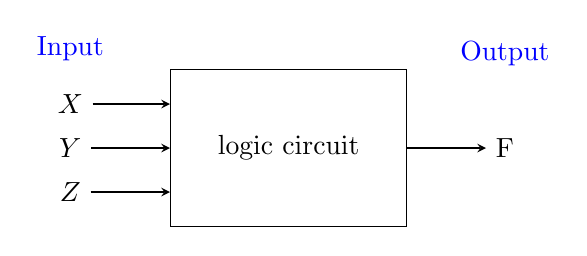
\begin{tikzpicture}[>=stealth,blk/.style={draw, minimum width=3cm, minimum height=2cm}]
\node (z) {$Z$};
\node (y) [above=2pt of z]{$Y$};
\node (x) [above=2pt of y]{$X$};
\node (Input) [above=5pt of x]{\textcolor{blue}{Input}};
\node (A) [right=of y,blk]{logic circuit};
\node (F) [right=of A]{F};
\node (blank) [above=2pt of F]{};
\node (Output) [above=10pt of blank]{\textcolor{blue}{Output}};
\draw [->] (x)--(A.west|-x);
\draw [->] (y)--(A);
\draw [->] (z)--(A.west|-z);
\draw [->] (A)--node[above]{}(F);
\end{tikzpicture}
\item A logic circuit whose outputs depend only on its current inputs is called a combinational circuit. The operation of such a circuit is fully described by a truth table that lists all combinations of input values and the corresponding output values. Below is an example of a truth table.\\
\begin{displaymath}
\begin{array}{c c c c}
\hline
X & Y & Z & F\\
\hline
0 & 0 & 0 & 0\\
0 & 0 & 1 & 1\\
0 & 1 & 0 & 0\\
0 & 1 & 1 & 0\\
1 & 0 & 0 & 0\\
1 & 0 & 1 & 0\\
1 & 1 & 0 & 1\\
1 & 1 & 1 & 1\\
\hline
\end{array}
\end{displaymath}
\item A circuit with memory whose outputs depend on the current input in addition to the sequence of past inputs are called sequential circuits. Its behavior may be described by a state table, which specifies its output and next state as functions of its current state and input. 
\item The most basic digital devices are called gates. Generally speaking, a gate has one or more inputs and produces an output that is a function of the current input values. 
\item Just three basic logic functions (AND, OR, and NOT) can be used to build any combinational logic circuit. The graphical symbols, along with their corresponding truth tables, are shown below.\\
\begin{circuitikz}
\ctikzset{tripoles/american and port/width=1}
\draw (0,0) node[and port] (myand) {}
(myand.in 1) node[anchor=east] {X}
(myand.in 2) node[anchor=east] {Y}
(myand.out)  node[right=1.4cm] (c) {}
(myand.out) node[anchor=south] {~~~~~~~~~~~X AND Y}
(myand.out) node[anchor=north] {~~~~~~~~~~~X$\cdot$Y}

(myand.out)  -- (c);
\end{circuitikz}
\begin{tabular}{c c c}
\hline
X & Y & X AND Y\\
\hline
0 & 0 & 0\\
0 & 1 & 0\\
1 & 0 & 0\\
1 & 1 & 1\\
\hline
\end{tabular}\\~\\~\\
\begin{circuitikz}
\ctikzset{tripoles/american and port/width=1}
\draw (0,0) node[and port] (myand) {}
(myand.in 1) node[anchor=east] {X}
(myand.in 2) node[anchor=east] {Y}
(myand.out)  node[right=1.4cm] (c) {}
(myand.out) node[anchor=south] {~~~~~~~~~~~X OR Y}
(myand.out) node[anchor=north] {~~~~~~~~~~~X+Y}

(myand.out)  -- (c);
\end{circuitikz}
\begin{tabular}{c c c}
\hline
X & Y & X OR Y\\
\hline
0 & 0 & 0\\
0 & 1 & 1\\
1 & 0 & 1\\
1 & 1 & 1\\
\end{tabular}\\~\\~\\
\begin{circuitikz}
\draw (0,0) node[not port] (mynot) {}
(mynot.in 1) node[anchor=east] {X}
(mynot.out)  node[right=1cm] (c) {}
(mynot.out) node[anchor=south] {~~~~~~NOT X}
(mynot.out) node[anchor=north] {~~~~~~X}

(mynot.out)  -- (c);
\end{circuitikz}
\begin{tabular}{c c}
\hline
X & NOT X\\
\hline
0 & 1\\
1 & 0\\
\end{tabular}\\
The gates' functions are easily described using words.
\begin{itemize}
\item An AND gate produces a 1 output if and only if all of its inputs are 1.
\item An OR gate produces a 1 output if and only if one or more of its inputs is 1.
\item A NOT gate is usually called an inverter and produces an output value the opposite of its input value.  
\end{itemize}
\item Take notice of the below circle from the inverter symbol's output.\\
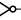
\includegraphics[scale=5]{IMG2}\\
This is called an inversion bubble and is used in this and other gate symbols to denote ``inverting'' behavior. 
\item Two additional logic functions are obtained by inverting the outputs of AND and OR gates. Shown below are their graphical symbols and their truth tables.\\
\begin{circuitikz}
\ctikzset{tripoles/american nand port/width=1}
\draw (0,0) node[nand port] (mynand) {}
(mynand.in 1) node[anchor=east] {X}
(mynand.in 2) node[anchor=east] {Y}
(mynand.out)  node[right=1.5cm] (c) {}
(mynand.out) node[anchor=south] {~~~~~~~~~~~X NAND Y}
(mynand.out) node[anchor=north] {~~~~~~~~~~~(X$\cdot$Y)$'$}

(mynand.out)  -- (c);
\end{circuitikz}
\begin{tabular}{c c c}
\hline
X & Y & X NAND Y\\
\hline
0 & 0 & 1\\
0 & 1 & 1\\
1 & 0 & 1\\
1 & 1 & 0\\
\hline
\end{tabular}\\~\\~\\
\begin{circuitikz}
\ctikzset{tripoles/american nor port/width=1}
\draw (0,0) node[nor port] (mynor) {}
(mynor.in 1) node[anchor=east] {X}
(mynor.in 2) node[anchor=east] {Y}
(mynor.out)  node[right=1.4cm] (c) {}
(mynor.out) node[anchor=south] {~~~~~~~~~~~X NOR Y}
(mynor.out) node[anchor=north] {~~~~~~~~~~~(X+Y)$'$}

(mynor.out)  -- (c);
\end{circuitikz}
\begin{tabular}{c c c}
\hline
X & Y & X NOR Y\\
\hline
0 & 0 & 1\\
0 & 1 & 0\\
1 & 0 & 0\\
1 & 1 & 0\\
\hline
\end{tabular}
\item A logic diagram shows the graphical symbols for multiple logic gates and other elements in a logic circuit, in addition to their interconnections (called wires). The output of each element may connect to inputs of one or more other elements. Signals in a logic diagram traditionally flow left to right, and inputs and outputs of the overall circuit are drawn on the left and right, respectively.\\
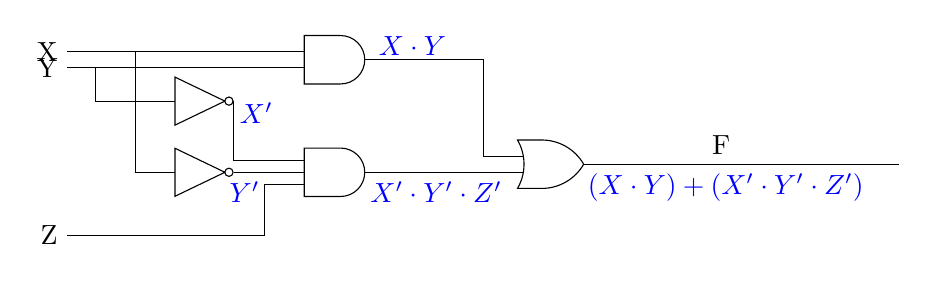
\begin{tikzpicture}[circuit logic US, node distance=8mm]
    \node[and gate] (and1) {};
    \draw (and1.input 1)--++(180:3cm) node[left] (X) {X};
    \draw (and1.input 2)--++(180:3cm) node[left] (Y) {Y};
    \node[and gate, below =of and1, logic gate inputs = nnn] (and2) {};
    \node[not gate, left=1cm of and2.input 2, scale=.85] (not1) {};
    \node[not gate, left=1cm of and2.input 1,yshift=7.5mm,scale=.85] (not2) {};
    \draw (not1.output) |- (and2.input 2);
    \draw (not2.output) |- (and2.input 1);
    \node[right=of not1, above, yshift=5mm, xshift=-4mm] (state3) {\textcolor{blue}{$X'$}};
    \node[right=of not1, below, xshift=-5.5mm] (state3) {\textcolor{blue}{$Y'$}};
    \draw (not1.input)--++(180:5mm) coordinate (aux) |- (X);
    \draw (not2.input)--++(180:10mm) coordinate (aux) |- (Y);
    \draw (and2.input 3)--++(180:5mm) |- ([yshift=-15mm]not2.south) coordinate (aux) -- (aux-|Y.east) node[left] (Z) {Z};
    \node[or gate, right=2cm of and2, anchor=input 2] (or2) {};
    \draw (and2)-|([xshift=-5mm]or2.input 2)--(or2.input 2) node[below, xshift=-1.1cm] (b) {\textcolor{blue}{$X'\cdot Y'\cdot Z'$}};
    \draw (and1)-|([xshift=-5mm]or2.input 1)--(or2.input 1) node[above, yshift=1.15cm, xshift=-1.4cm] (a) {\textcolor{blue}{$X\cdot Y$}};
    \draw (or2.output)--++(0:4cm);
    \node[right=of or2, above] (state1) {~~~~~~~~~~~~~~~~F};
    \node[right=of or2, below] (state2) {~~~~~~~~~~~~~~~~~\textcolor{blue}{$(X\cdot Y)+(X'\cdot Y'\cdot Z')$}};
\end{tikzpicture}
\item Besides voltage and current, logic circuits are also useful in representing time. A timing function graphically hows how a circuit may respond to a time-varying pattern of various input signals. Time is graphed horizontally and logic values are graphed vertically. 
\item By obtaining a formal definition of a combinational circuit's logic function, we can analyze it. This description allows us to perform a variety of operations, such as determining the logic circuit's behavior, manipulating an algebraic or equivalent graphical description to suggest different circuit elements for the logic function, and more. 
\item Given a logic diagram for a combinational circuit, there are several ways to obtain a formal description of the circuit's function, the most basic of which is the truth table.
\item Using only the basic axioms of switching algebra, we can easily obtain the truth table of an $n$-input circuit by working our way through all $2^n$ input combinations. For each input combination, we determine each of the gate outputs produced by the input and propagate information from the circuit inputs to outputs. 
\item The number of input combinations for a logic circuit grows exponentially in relation to the number of inputs, so an exhaustive approach such as the one described above can become tiring. Because of this, for many analysis problems it is better to use an algebraic approach whose complexity is more linearly proportional to the size of the circuit.
\item This new method is simple: we build up a parenthesized logic expression corresponding to the logic operators and the structure of the circuit. We start at the inputs and propagate expressions as we move toward the output. You can either simplify these expressions using the axioms of switching algebra as you go or all at once at the end. 
\end{itemize}\pagebreak
\section{2/14/2020}
\subsection{Lecture Slides}
\begin{itemize}
\item Problem 9.1.1: Take the dual of $Y=X+W'T+WT'$.\\
We must swap $\cdot\to+$ and $+\to\cdot$. There are no zeros or ones so we don't need to worry about swapping those.\\
\answer{Dual of $Y=X\cdot(W'+T)\cdot(W+T')$}
\item Problem 9.1.2: Take the dual of $F=A'B+ABC'$.\\
We must swap $\cdot\to+$ and $+\to\cdot$. There are no zeros or ones so we don't need to worry about swapping those.\\
\answer{Dual of $F=(A'+B)\cdot(A+B+C')$}
\item With canonical representation, every term in our equation contains every input. 
\item In SOP, or Sum of Products, each term is the product of the literals and they are all summed together. In a truth table, if the input for a literal for that minterm is a 1, then the literal is itself. Conversely, if the input for a literal for that minterm is a 0, then the literal is a complement of itself. Since SOP is a sum, we represent it with $\sum_{\text{variables in the function}}$.
\item POS, or Product of Sums, is when each term is summed together and then is taken as the product. In a truth table, if the input for a literal for that maxterm is a 1, then the literal is a complement of itself. Conversely, if the input for a literal for that maxterm is a 0, then the literal is the complement of itself. We use the capital greek letter pi, or $\prod$, to represent POS. 
\item Because functions can get long, we use shorthand to make writing them more manageable. When writing a function, just write which minterm or maxterm numbers to include. Furthermore, use $\sum$ for SOP (also known as sigma notation) and $\prod$ for POS (also known as pi notation). 
\item Problem 9.1.3: Create the truth table for $F=\sum(2,4,6,7)$.\\
\begin{displaymath}
\begin{array}{|c c c|c|}
x & y & z & F\\
\hline
0 & 0 & 0 & 0\\
0 & 0 & 1 & 0\\
0 & 1 & 0 & 1\\
0 & 1 & 1 & 0\\
1 & 0 & 0 & 1\\
1 & 0 & 1 & 0\\
1 & 1 & 0 & 1\\
1 & 1 & 1 & 1\\
\end{array}
\hspace{.5cm}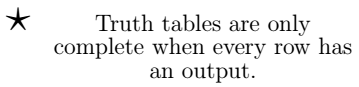
\includegraphics{IMG1}
\end{displaymath}~\\
\item Problem 9.1.4: Create the truth table for $F=\sum(0,5,6)$.\\
\begin{displaymath}
\begin{array}{|c c c|c|}
x & y & z & F\\
\hline
0 & 0 & 0 & 1\\
0 & 0 & 1 & 0\\
0 & 1 & 0 & 0\\
0 & 1 & 1 & 0\\
1 & 0 & 0 & 0\\
1 & 0 & 1 & 1\\
1 & 1 & 0 & 1\\
1 & 1 & 1 & 0\\
\end{array}
\end{displaymath}
\item Problem 9.1.5: Create the canonical function for $\sum(2,4,6,7)$.\\
Using a truth table, find the values of 2, 4, 6, and 7. 2 is 010, 4 is 100, 6 is 110, and 7 is 111. Next, convert these into the canonical function using x, y, and z.\\
\answer{$F=\overline{x}y\overline{z}+x\overline{y}\overline{z}+xy\overline{z}+xyz$}
\item Problem 9.1.6: Create the canonical function for $\sum(0,5,6)$.\\
Using a truth table, find the values of 0, 5, and 6. 0 is 000, 5 is 101, and 6 is 110. Next, convert these into the canonical function using x, y, and z.\\
\answer{$F=\overline{xyz}+x\overline{y}+xy\overline{z}$}
\item Problem 9.1.7: Create the truth table for $F=\prod(2,4,6,7)$.\\
\begin{displaymath}
\begin{array}{|c c c|c|}
x & y & z & F\\
\hline
0 & 0 & 0 & 1\\
0 & 0 & 1 & 1\\
0 & 1 & 0 & 0\\
0 & 1 & 1 & 1\\
1 & 0 & 0 & 0\\
1 & 0 & 1 & 1\\
1 & 1 & 0 & 0\\
1 & 1 & 1 & 0\\
\end{array}
\end{displaymath}
\item Problem 9.1.8: Create the truth table for $F=\prod(0,5,6)$.
\begin{displaymath}
\begin{array}{|c c c|c|}
x & y & z & F\\
\hline
0 & 0 & 0 & 0\\
0 & 0 & 1 & 1\\
0 & 1 & 0 & 1\\
0 & 1 & 1 & 1\\
1 & 0 & 0 & 1\\
1 & 0 & 1 & 0\\
1 & 1 & 0 & 0\\
1 & 1 & 1 & 1\\
\end{array}
\end{displaymath}
\item Problem 9.1.9: Create the canonical function for $F=\prod(2,4,6,7)$.\\
Using a truth table, find the values of 2, 4, 6, and 7. 2 is 010, 4 is 100, 6 is 110, and 7 is 111. Next, convert these into the canonical function using x, y, and z.\\
\answer{$F=(x+y+\ol{z})(\ol{x}+y+z)(\ol{x}+\ol{y}+\ol{z})(\ol{x}+\ol{y}+z)$}
\item Problem 9.1.10: Create the canonical function for $F=\prod(0,5,6)$.\\
Using a truth table, find the values of 0, 5, and 6. 0 is 000, 5 is 101, and 6 is 110. Next, convert these into the canonical function using x, y, and z.\\
\answer{$F=(x+y+z)(\ol{x}+y+z)(\ol{x}+\ol{y}+z)$}
\item On-set and off-set is a system used to describe the shorthand list of items. Minterms in shorthand have a list of the rows with 1 as the output, making it on-set. The complementary idea also holds true, with off-set being for maxterms. 
\item Logic gates are used to physically represent functions and can be drawn. AND, OR, and NOT are said to create a complete logic set.\\
\item Logic diagrams are drawings that help with design and preparation for implementation. For now, we will only use computational logic.\\
\item Multi level and two level are forms of canonical representation systems. Two level is SOP or POS form. NOTs don't count. Unless explicitly told otherwise, always simplify and create a SOP style.
\item Problem 9.1.11: Draw the logic diagram for $F=AB'+B'C$.\\
\begin{tikzpicture}[circuit logic US, node distance=8mm]
	\node[and gate] (and1) {};
    \draw (and1.input 1)--++(180:3cm) node[left] (A) {A};
    \node[below= of A] (B) {B};
    \node[not gate, right=1.5cm of B,scale=.85] (not1) {};
    \node[below= of B] (C) {C};
    \draw (not1.input)--++(180:5mm) coordinate (aux) |- (B);
    \node[and gate, right=3cm of C] (and2) {};
    \draw (and2.input 1)--++(180:5mm) coordinate (aux) |- (not1.output);
    \draw (and1.input 2)--++(180:5mm) coordinate (aux) |- (not1.output);
    \draw (and2.input 2)--++(180:5mm) coordinate (aux) |- (C);
    \node[or gate, right=3cm of not1] (or1) {};
    \draw (or1.input 1)--++(180:5mm) coordinate (aux) |- (and1.output);
    \draw (or1.input 2)--++(180:5mm) coordinate (aux) |- (and2.output);
    \node[right=.75cm of or1] (F) {F};
    \draw (or1.output) |- (F);
\end{tikzpicture}
\item Problem 9.1.12: Draw the logic diagram for $T=MX+B'X'$.\\
\begin{tikzpicture}[circuit logic US, node distance=8mm]
	\node[and gate] (and1) {};
    \draw (and1.input 1)--++(180:3cm) node[left] (M) {M};
    \node[below= of A] (B) {B};
    \node[not gate, right=1.5cm of B,scale=.85] (not1) {};
    \draw (not1.input)--++(180:5mm) coordinate (aux) |- (B);
    \node[below= of B] (X) {X};
    \node[not gate, right=1.5cm of X,scale=.85] (not2) {};
    \draw (not2.input)--++(180:5mm) coordinate (aux) |- (X);
    \node[and gate, below=1.1cm of and1] (and2) {};
    \draw (and2.input 1)--++(180:5mm) coordinate (aux) |- (not1.output);
    \draw (and2.input 2)--++(180:5mm) coordinate (aux) |- (not2.output);
    \node[or gate, right=4.5cm of B, yshift=.55cm] (or1) {};
    \draw (or1.input 1)--++(180:5mm) coordinate (aux) |- (and1.output);
    \draw (or1.input 2)--++(180:5mm) coordinate (aux) |- (and2.output);
    \node[right=.75cm of or1] (T) {T};
    \draw (or1.output) |- (T);
\end{tikzpicture}
\end{itemize}
\subsection{Assigned Reading}
\begin{itemize}
\item A logic circuit description is occasionally just a list of input combinations for when a signal would be on or off. For example, the description of a 4-bit prime-number detector might be ``Given a 4-bit input combination $N=N_3N_2N_1N_0$, produce a 1 output for $N=1,2,3,5,7,11,13$.''\pagebreak
\item A logic function described in this way can be designed directly from a given canonical sum or produce expression. For the above prime-number detector, we would have...\\
$F=\sum_{N_3,N_2,N_1,N_0}(1,2,3,5,7,11,13)$\\
$\textcolor{white}{F}=N_3'\cdot N_2'\cdot N_1'\cdot N_0+N_3'\cdot N_2'\cdot N_1\cdot N_0'+N_3'\cdot N_2'\cdot N_1\cdot N_0+N_3'\cdot N_2\cdot N_1'\cdot N_0+N_3'\cdot N_2\cdot N_1\cdot N_0+N_3\cdot N_2'\cdot N_1\cdot N_0+N_3\cdot N_2\cdot N_1'\cdot N_0$
\item More often than this, however, we describe a logic function using the natural-language connections ``and'', ``or'', and ``not.'' For example, we might describe an alarm circuit by saying 
\begin{displayquote}
``The ALARM output is 1 if the PANIC input is 1, or if the ENABLE input is 1, the EXITING input is 0, and the house is not secure; the house is secure if the WINDOW, DOOR, and GARAGE inputs are all 1.''
\end{displayquote}
Such a description can be directly translated into algebraic expressions.
\begin{displayquote}
$\text{ALARM}=\text{PANIC}+\text{ENABLE}\cdot\text{EXITING}'\cdot\text{SECURE}'$\\
$\text{SECURE}=\text{WINDOW}\cdot\text{DOOR}\cdot\text{GARAGE}$\\
$\text{ALARM}=\text{PANIC}+\text{ENABLE}\cdot \text{EXITING}'\cdot(\text{WINDOW}\cdot\text{DOOR}\cdot\text{GARAGE})$
\end{displayquote}
\item A circuit realizes an expression if its output function equals that expression. If a circuit realizes an expression, it is called a realization of the function. In place of realization, the term ``implementation'' is sometimes used. Recognize both - they are both used in practice.
\item Once we have any expression, we can do more than just build a circuit from the expression. We can, for example, manipulate the expression to get different circuits. The aforementioned ALARM expression can be multiplied out to get a sum-of-products circuit, as an example. Alternatively, if the number of variables isn't very large, we can create a truth table for the expression.
\item In general, when we are designing a logic function for an application, it is easier to describe the logic function in words using logical connectives than it is to write a complete truth table (especially if the number of variables is large). 
\item Sometimes however we start with imprecise word descriptions of logic functions, such as the sentence ``The ERROR output should be 1 if the GEARUP, GEARDOWN, and GEARCHECK inputs are inconsistent.'' In these cases, a truth-table approach is more optimal because it allows us to determine the output required for every input. Using a logic expression in this case might make it difficult to notice ``corner cases'' and handle them appropriately. 
\end{itemize}\pagebreak
\section{2/17/2020}
\subsection{Lecture Slides}
\begin{itemize}
\item Problem 10.1.1: Draw the logic diagram for $T=MX+BM'+X'$. 
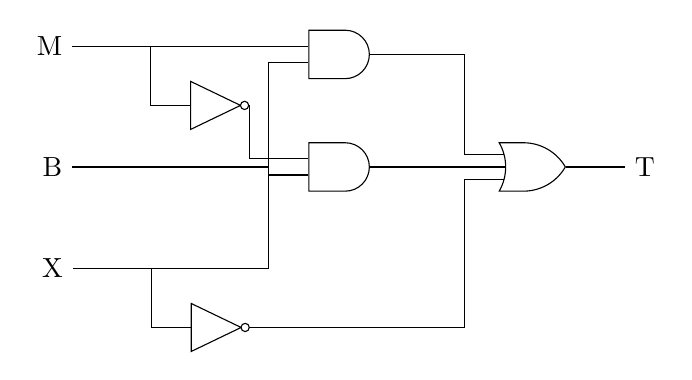
\begin{tikzpicture}[circuit logic US, node distance=8mm]
	\node[and gate] (and1) {};
    \draw (and1.input 1)--++(180:3cm) node[left] (M) {M};
    \node [not gate, right=1.5cm of M, yshift=-.75cm, scale=.85] (not1) {};
    \node[and gate, below=of and1] (and2) {};
    \node[left=3cm of and2] (B) {B};
    \draw (not1.output) |- (and2.input 1);
    \draw (and2.input 2)--++(180:5mm) coordinate (aux) |- (B);	
    \draw (not1.input)--++(180:5mm) coordinate (aux) |- (M);	
    \node[below= of B] (X) {X};
    \node [not gate, right=1.5cm of X, yshift=-.75cm, scale=.85] (not2) {};
    \draw (and1.input 2)--++(180:5mm) coordinate (aux) |- (X);
    \draw (not2.input)--++(180:5mm) coordinate (aux) |- (X);
    \node[or gate, right=5.5cm of B, logic gate inputs = nnn] (or1) {};
	\draw (or1.input 1)--++(180:5mm) coordinate (aux) |- (and1.output);    
	\draw (or1.input 2)--++(180:5mm) coordinate (aux) |- (and2.output);
	\draw (or1.input 3)--++(180:5mm) coordinate (aux) |- (not2.output);
	\node[right=.75cm of or1] (T) {T};
    \draw (or1.output) |- (T);
\end{tikzpicture}
\item Problem 10.1.2: Draw the logic diagram for $T=X'+B(X'+C)$. \\
\begin{tikzpicture}[circuit logic US, node distance=8mm]
	\node[] (X) {X};
	\node [not gate, right=1.5cm of X, scale=.85] (not1) {};
	\draw (not1.input)--++(180:5mm) coordinate (aux) |- (X);
	\node[below=of X] (B) {B};
	\node[below=of B] (C) {C};
	\node[or gate, right=3cm of B, yshift=.5cm] (or1) {};
	\draw (or1.input 1)--++(180:5mm) coordinate (aux) |- (not1);
	\draw (or1.input 2)--++(180:5mm) coordinate (aux) |- (C);
	\node[and gate, right=5cm of B] (and1) {};
	\draw (and1.input 1)--++(180:5mm) coordinate (aux) |- (or1.output);
	\draw (and1.input 2)--++(180:5mm) coordinate (aux) |- (B);
	\node[or gate, right=2cm of and1] (or2) {};
	\draw (or2.input 1)--++(180:5mm) coordinate (aux) |- (not1.output);
	\draw (or2.input 2)--++(180:5mm) coordinate (aux) |- (and1.output);
	\node[right=.75cm of or2] (T) {T};
    \draw (or2.output) |- (T);
\end{tikzpicture}
\item You can always follow the path of connections in a diagram to see the behavior that it is implementing. This is done by labeling the function after each gate. See the below problems for examples. 
\item Problem 10.1.3: Develop the equation for the logic diagram. Do not simplify the solution.\\
\begin{tikzpicture}[circuit logic US, node distance=8mm]
	\node[] (A) {A};
	\node [not gate, right=1.5cm of A, scale=.85] (not1) {};
	\draw (not1.input)--++(180:5mm) coordinate (aux) |- (A);
	\node[below=of A] (B) {B};
	\node[below=of B] (C) {C};
	\node[below=of C] (D) {D};
	\node[and gate,below=1.3cm of not1] (and1) {};
	\node [not gate, right=1.5cm of D, scale=.85] (not2) {};
	\draw (not2.input)--++(180:5mm) coordinate (aux) |- (D);
	\draw (and1.input 1)--++(180:5mm) coordinate (aux) |- (B);
	\draw (and1.input 2)--++(180:5mm) coordinate (aux) |- (C);
	\node [or gate, right=3cm of A, yshift=-.75cm] (or1) {};
	\draw (or1.input 1)--++(180:5mm) coordinate (aux) |- (not1) node[above, xshift=.75cm] (state2) {$A'$};
	\draw (or1.input 2)--++(180:5mm) coordinate (aux) |- (and1) node[below, xshift=.75cm] (state3) {$B\cdot C$};
	\node[or gate, right=3cm of and1] (or2) {};
	\draw (or2.input 1)--++(180:5mm) coordinate (aux) |- (or1.output) node[above, xshift=1cm] (state1) {$(A'+(B\cdot C))$};
	\draw (or2.input 2)--++(180:5mm) coordinate (aux) |- (not2) node[above, xshift=1cm] (state1) {$D'$};
	\node[right=.75cm of or2] (M) {$M=(A'+(B\cdot C))+D'$};
    \draw (or2.output) |- (M);
\end{tikzpicture}\pagebreak
\item Problem 10.1.4: Develop the equation for the logic diagram. Do not simplify the solution.\\
\begin{tikzpicture}[circuit logic US, node distance=8mm]
	\node[] (A) {A};
	\node [not gate, right=1.5cm of A, scale=.85] (not1) {};
	\draw (not1.input)--++(180:5mm) coordinate (aux) |- (A);
	\node[below=of A] (B) {B};
	\node[below=of B] (C) {C};
	\node[below=of C] (D) {D};
	\node[and gate,below=1.3cm of not1] (and1) {};
	\node [not gate, right=1.5cm of D, scale=.85] (not2) {};
	\draw (not2.input)--++(180:5mm) coordinate (aux) |- (D);
	\draw (and1.input 1)--++(180:5mm) coordinate (aux) |- (B);
	\draw (and1.input 2)--++(180:5mm) coordinate (aux) |- (C);
	\node[and gate, right=3cm of D, yshift=1cm] (and2) {};
	\draw (and2.input 1)--++(180:5mm) coordinate (aux) |- (and1.output) node[above, xshift=.45cm] (state3) {$B\cdot C$};
	\draw (and2.input 2)--++(180:5mm) coordinate (aux) |- (not2.output) node[below, xshift=.25cm] (state1) {$D'$};
	\node[or gate, right=3cm of and1, yshift=.5cm] (or1) {};
	\draw (or1.input 1)--++(180:5mm) coordinate (aux) |- (not1.output) node[above, xshift=.75cm] (state2) {$A'$};
	\draw (or1.input 2)--++(180:5mm) coordinate (aux) |- (and2.output) node[below, xshift=.85cm] (state4) {$(B\cdot C)\cdot D'$};
	\node[right=.75cm of or1] (M) {$M=A'+((B\cdot C)\cdot D')$};
    \draw (or1.output) |- (M);
\end{tikzpicture}
\item Combinational logic synthesis is the process that specifies the required function and creates the details for implementation. Combinational logic design is the broader overview of the entire process, which includes logic synthesis. 
\end{itemize}\pagebreak
\section{2/19/2020}
\subsection{Lecture Slides}
\begin{itemize}
\item A manipulator is a fancy way of saying that we can make an equivalent function with different arrangements. 
\item Problem 11.1.1: Draw the canonical logic diagram for $F=\sum_{x,y,z}(2,4,6)$ but with only two input gates and NOTs.\\
\begin{tikzpicture}[circuit logic US, node distance=8mm]
	\node[] (X) {X};
	\node [not gate, right=1.5cm of X, yshift=-.75cm, scale=.85] (not1) {};
	\draw (not1.input)--++(180:5mm) coordinate (aux) |- (X);
	\node[below=of X] (Y) {Y};
	\node[below=of Y] (Z) {Z};
	\node [not gate, right=1.5cm of Y, yshift=-.75cm, scale=.85] (not2) {};
	\draw (not2.input)--++(180:5mm) coordinate (aux) |- (Y);
	\node [not gate, right=1.5cm of Z, yshift=-.75cm, scale=.85] (not3) {};
	\draw (not3.input)--++(180:5mm) coordinate (aux) |- (Z);
	\node[and gate, right=3.5cm of A, logic gate inputs = nnn] (and1) {};
	\node[and gate, right=3.5cm of B, logic gate inputs = nnn] (and2) {};
	\node[and gate, right=3.5cm of C, logic gate inputs = nnn] (and3) {};
	\node[or gate, right=1.5cm of and2] (or1) {};
	\draw (and1.input 1)--++(180:5mm) coordinate (aux) |- (not1.output);
	\draw (and2.input 2)--++(180:5mm) coordinate (aux) |- (not2.output);
	\draw (and3.input 3)--++(180:5mm) coordinate (aux) |- (not3.output);
	\draw (and1.input 2)--++(180:5mm) coordinate (aux) |- (Y);
	\draw (and1.input 3)--++(180:5mm) coordinate (aux) |- (not3.output);
	\draw (and2.input 1)--++(180:5mm) coordinate (aux) |- (X);
	\draw (and2.input 3)--++(180:5mm) coordinate (aux) |- (not3.output);
	\draw (and3.input 1)--++(180:5mm) coordinate (aux) |- (X);
	\draw (and3.input 2)--++(180:5mm) coordinate (aux) |- (Y);
	\draw (or1.input 1)--++(180:5mm) coordinate (aux) |- (and1.output);
	\draw (or1.input 2)--++(180:5mm) coordinate (aux) |- (and2.output);
	\draw (or1.input 3)--++(180:5mm) coordinate (aux) |- (and3.output);
	\node[right=.75cm of or1] (F) {F};
    \draw (or1.output) |- (F);
\end{tikzpicture}\\
This is a two level, three input gate $F=\ol{x}y\ol{z}+x\ol{yz}+xy\ol{z}$. Using the associative property, we can create a multi-level two input gate $F=\ol{z}(\ol{x}y+x\ol{y}+xy)$.\\ 
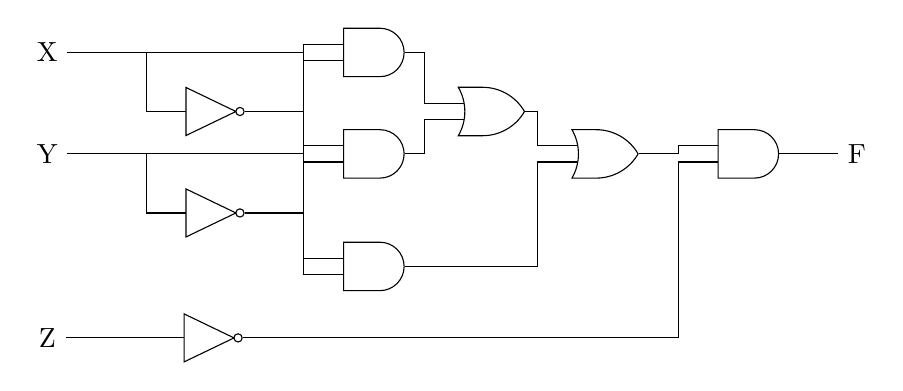
\begin{tikzpicture}[circuit logic US, node distance=8mm]
	\node[] (X) {X};
	\node [not gate, right=1.5cm of X, yshift=-.75cm, scale=.85] (not1) {};
	\draw (not1.input)--++(180:5mm) coordinate (aux) |- (X);
	\node[below=of X] (Y) {Y};
	\node[below=of Y] (invisible) {};
	\node[below=of invisible] (Z) {Z};
	\node [not gate, right=1.5cm of Y, yshift=-.75cm, scale=.85] (not2) {};
	\draw (not2.input)--++(180:5mm) coordinate (aux) |- (Y);
	\node [not gate, right=1.5cm of Z, scale=.85] (not3) {};
	\draw (not3.input)--++(180:5mm) coordinate (aux) |- (Z);
	\node[and gate, right=3.5cm of X] (and1) {};
	\node[and gate, right=3.5cm of Y] (and2) {};
	\node[and gate, below= of and2] (and3) {};
	\draw (and1.input 1)--++(180:5mm) coordinate (aux) |- (not1.output);
	\draw (and1.input 2)--++(180:5mm) coordinate (aux) |- (Y);
	\draw (and2.input 1)--++(180:5mm) coordinate (aux) |- (X);
	\draw (and2.input 2)--++(180:5mm) coordinate (aux) |- (not2.output);
	\draw (and3.input 1)--++(180:5mm) coordinate (aux) |- (X);
	\draw (and3.input 2)--++(180:5mm) coordinate (aux) |- (Y);
	\node[or gate, right=2.9cm of not1] (or1) {};
	\draw (or1.input 1)--++(180:5mm) coordinate (aux) |- (and1.output);
	\draw (or1.input 2)--++(180:5mm) coordinate (aux) |- (and2.output);
	\node[or gate, right=2.2cm of and2] (or2) {};
	\draw (or2.input 1)--++(180:5mm) coordinate (aux) |- (or1.output);
	\draw (or2.input 2)--++(180:5mm) coordinate (aux) |- (and3.output);
	\node[and gate, right=1cm of or2] (and4) {};
	\draw (and4.input 1)--++(180:5mm) coordinate (aux) |- (or2.output);
	\draw (and4.input 2)--++(180:5mm) coordinate (aux) |- (not3.output);
	\node[right=.75cm of and4] (F) {F};
    \draw (and4.output) |- (F);
\end{tikzpicture}
\item Problem 11.1.2: Draw the canonical logic diagram for $F=\sum_{x,y,z}(1,5)$ but only with two input gates and NOTs.\\
\begin{tikzpicture}[circuit logic US, node distance=8mm]
	\node[] (X) {X};
	\node [not gate, right=1.5cm of X, yshift=-.55cm, scale=.85] (not1) {};
	\draw (not1.input)--++(180:5mm) coordinate (aux) |- (X);
	\node[below=of X] (Y) {Y};
	\node [not gate, right=1.5cm of Y, scale=.85] (not2) {};
	\draw (not2.input)--++(180:5mm) coordinate (aux) |- (Y);
	\node[below=of Y] (Z) {Z};
	\node[and gate, right=3.5cm of X,yshift=-.5cm] (and1) {};
	\node[and gate, right=3.5cm of Z,yshift=.5cm] (and2) {};
	\draw (and1.input 1)--++(180:5mm) coordinate (aux) |- (not1.output);
	\draw (and1.input 2)--++(180:5mm) coordinate (aux) |- (not2.output);
	\draw (and1.input 3)--++(180:5mm) coordinate (aux) |- (Z);
	\draw (and2.input 1)--++(180:5mm) coordinate (aux) |- (X);
	\draw (and2.input 2)--++(180:5mm) coordinate (aux) |- (not2.output);
	\draw (and2.input 3)--++(180:5mm) coordinate (aux) |- (Z);
	\node[or gate, right=5.5cm of Y] (or1) {};
	\draw (or1.input 1)--++(180:5mm) coordinate (aux) |- (and1.output);
	\draw (or1.input 2)--++(180:5mm) coordinate (aux) |- (and2.output);
	\node[right=.75cm of or1] (F) {F};
    \draw (or1.output) |- (F);
\end{tikzpicture}\\
This above logic diagram is for $F=\ol{xy}z+x\ol{y}z$ and is incorrect. The below correct logic diagram takes advantage of the distributive property. $F=\ol{x}(\ol{y}z)+x(\ol{y}z)$.\\	
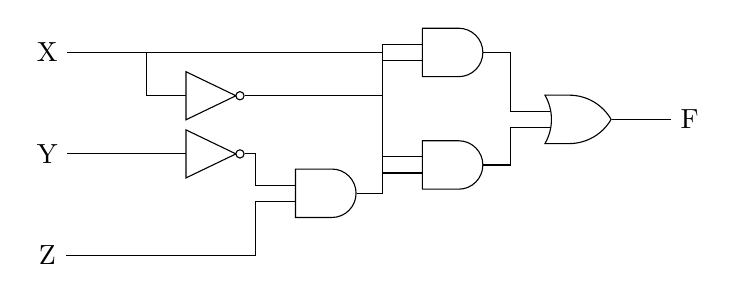
\begin{tikzpicture}[circuit logic US, node distance=8mm]
	\node[] (X) {X};
	\node [not gate, right=1.5cm of X, yshift=-.55cm, scale=.85] (not1) {};
	\draw (not1.input)--++(180:5mm) coordinate (aux) |- (X);
	\node[below=of X] (Y) {Y};
	\node [not gate, right=1.5cm of Y, scale=.85] (not2) {};
	\draw (not2.input)--++(180:5mm) coordinate (aux) |- (Y);
	\node[below=of Y] (Z) {Z};
	\node[and gate, right=4cm of X, xshift=.5cm] (and1) {};
	\node[and gate, right=.75cm of not2, yshift=-.5cm] (and2) {};
	\node[and gate, below=of and1] (and3) {};
	\draw (and2.input 1)--++(180:5mm) coordinate (aux) |- (not2.output);
	\draw (and2.input 2)--++(180:5mm) coordinate (aux) |- (Z);
	\draw (and1.input 1)--++(180:5mm) coordinate (aux) |- (not1.output);
	\draw (and1.input 2)--++(180:5mm) coordinate (aux) |- (and2.output);
	\draw (and3.input 1)--++(180:5mm) coordinate (aux) |- (X);
	\draw (and3.input 2)--++(180:5mm) coordinate (aux) |- (and2.output);
	\node[or gate, right=4cm of not1,yshift=-.3cm] (or1) {};
	\draw (or1.input 1)--++(180:5mm) coordinate (aux) |- (and1.output);
	\draw (or1.input 2)--++(180:5mm) coordinate (aux) |- (and3.output);
	\node[right=.75cm of or1] (F) {F};
    \draw (or1.output) |- (F);
\end{tikzpicture}
\item When designing a system, there are a few important questions to ask. 
\begin{itemize}
\item What are the inputs?
\item What are the outputs?
\item Are there any constraints or relationships between the inputs and outputs?
\end{itemize}
After asking these questions, you can build the design.
\item Problem 11.1.3: Design a system to turn on and off a sprinkler in the yard.\\
Inputs: Time(day$^1$ or night$^0$)$\to $T\\
\textcolor{white}{Inputs: }Weather (rain$^1$ or no rain$^0$)$\to $W\\~\\
Sprinkler: On$^1$ or off $^0=\text{output}\to$S\\~\\
\begin{tabular}{|cc|c|}
T & W & S\\
\hline
0 & 0 & 1\\
0 & 1 & 0\\
1 & 0 & 0\\
1 & 1 & 0\\
\end{tabular} $S=\ol{T}\cdot\ol{W}$\\
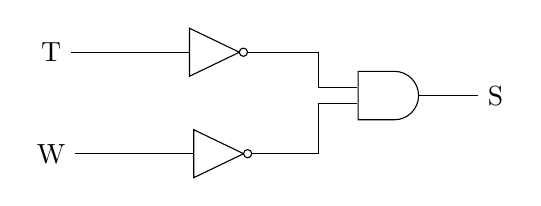
\begin{tikzpicture}[circuit logic US, node distance=8mm]
	\node[] (T) {T};
	\node[below=of T] (W) {W};
	\node [not gate, right=1.5cm of T, scale=.85] (not1) {};
	\draw (not1.input)--++(180:5mm) coordinate (aux) |- (T);
	\node [not gate, right=1.5cm of W, scale=.85] (not2) {};
	\draw (not2.input)--++(180:5mm) coordinate (aux) |- (W);
	\node[and gate, right=1.5cm of not1, yshift=-.55cm] (and1) {};
	\draw (and1.input 1)--++(180:5mm) coordinate (aux) |- (not1.output);
	\draw (and1.input 2)--++(180:5mm) coordinate (aux) |- (not2.output);
	\node[right=.75cm of and1] (S) {S};
    \draw (and1.output) |- (S);
\end{tikzpicture}
\item Problem 11.1.4: Design a system to determine if you are allowed to watch Netflix.\\
Inputs: Homework (have$^1$ or have not$^0$)$\to$H\\
\textcolor{white}{Inputs: }Class (in class$^1$ or not in class$^0$)$\to$C\\
Output: Watch Netflix (yes$^1$ or no$^0$)$\to$N\\~\\
\begin{tabular}{|cc|cc|}
H & C & N & \\
\hline
0 & 0 & 1 & \textcolor{red}1\\
0 & 1 & 0 & \textcolor{red}0\\
1 & 0 & 0 & \textcolor{red}1\\
1 & 1 & 0 & \textcolor{red}0\\
\end{tabular}\\
$N=\ol{H}\cdot\ol{C}$\\$\ol{H}\cdot\ol{C}=N$\\~\\
$N=\ol{H}\cdot\ol{C}+H\ol{C}=\ol{C}$\\
\end{itemize}
\section{2/21/2020}
\subsection{Lecture Slides}
\begin{itemize}
\item When solving logic systems, we usually want to take the lazier approach, so we look for methods that are simpler with less spots for error and a lower price to implement. 
\item Minimization aims to reduce the ``cost'', which is done by reducing the number and size of gates.
\item There are three key ways to reduce cost.
\begin{enumerate}
\item [1.] Minimize the number of first-level gates.
\item [2.] Minimize the number of inputs on each first level gate.
\item [3.] Minimize the number of inputs on each second level gate. 
\end{enumerate}
\item How are you handle how many inputs to use for a gate? Do as you're told, do as you're equipped to handle, and do as you want (in that order). 
\item Problem 12.1.1: Find the simplified POS $F=\prod_{x,y,z}(1,2,5,6)$.\\
$F=(x+y+\ol{z})(x+\ol{y}+z)(\ol{x}+y+\ol{z})(\ol{x}+\ol{y}+z)$\\
$F=(\cancel{xx}^x+x\ol{y}+xz+yx+\cancel{y\ol{y}}^0+yz+\ol{z}x+\ol{z}x+\cancel{\ol{z}z)}^0$\\
$\textcolor{white}{F=}(\cancel{\ol{xx}}^x+\ol{xy}+y\ol{x}+\cancel{y\ol{y}}^0+yz+\ol{zx}+\ol{zy}+\cancel{\ol{z}z}^0)$\\
$F=x\ol{x}+x\ol{xy}+x\ol{x}z+xy\ol{z}+xyz+x\ol{zx}+x\ol{zy}$\\
This takes too long! For POS functions, simplifying them algebraically is far too complicated. We need an alternative. 
\item Instead of solving algebraically, we use Karnaugh maps. Some Karnaugh maps are shown below.\\
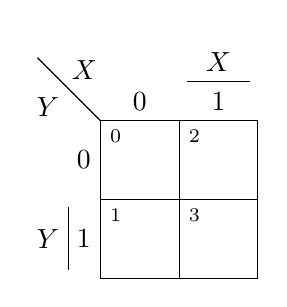
\begin{tikzpicture}
\karnaughmap[variables={XY}, function={}]{4};
\end{tikzpicture}\\
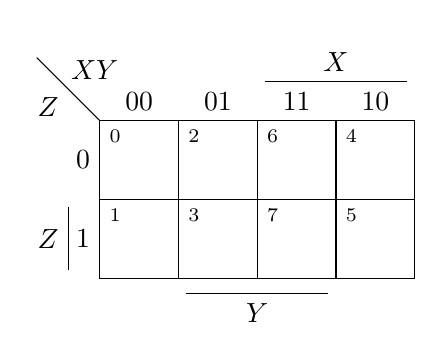
\begin{tikzpicture}
\karnaughmap[variables={XYZ}, function={}]{8};
\end{tikzpicture}\\
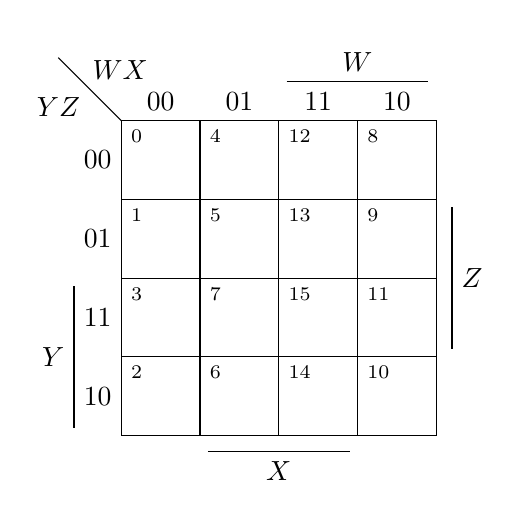
\begin{tikzpicture}
\karnaughmap[variables={WXYZ}, function={}]{16};
\end{tikzpicture}
\item There are a few things to note about K-Maps. First, working with more than four variables generally isn't worth it, at which computer aided design begins to be used. Second, the order of the numbers is in gray code. 
\item Why gray code? Take the two terms $A'BC+ABC$. If we apply the distributive property we get $BC(A'+A)$. Then, we can apply the complement theorem to get $(A'+A)=1$, which reduces to just $BC$. This can be interpreted from the K-Map through gray code, forcing terms that can cancel to be adjacent. 
\item Problem 12.1.2: How does the below truth table map to a K-Map?\\
\begin{tabular}{cc|c}
x & y & F\\
\hline
0 & 0 & A\\
0 & 1 & B\\
1 & 0 & C\\
1 & 1 & D\\
\end{tabular}\\
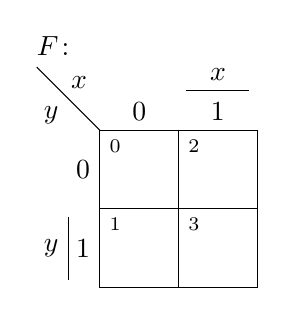
\begin{tikzpicture}
\karnaughmap[variables={xy}, function={F}]{4};
\end{tikzpicture}
\item Problem 12.1.3: How does the below truth table map to a K-Map?\\
\begin{tabular}{ccc|c}
x & y & z & F\\
\hline
0 & 0 & 0 & A\\
0 & 0 & 1 & B\\
0 & 1 & 0 & C\\
0 & 1 & 1 & D\\
1 & 0 & 0 & E\\
1 & 0 & 1 & F\\
1 & 1 & 0 & G\\
1 & 1 & 1 & H\\
\end{tabular}\\
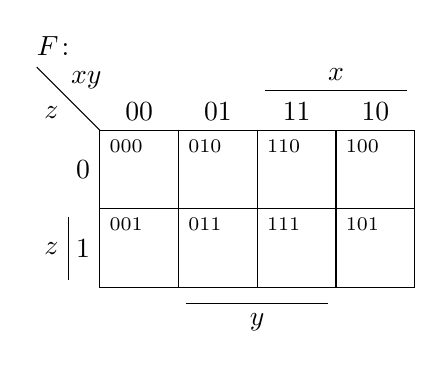
\begin{tikzpicture}
\karnaughmap[variables={xyz}, function={F}, binaryidx]{8};
\end{tikzpicture}
\item To use the K-Map for reduction, some vocabulary terms need to get defined.
\begin{itemize}
\item Implicants (or a covers) are power of 2 circles/rectangles that go around neighboring 1's in SOP and 0's in POS. The prime implicant, or PI, is the largest cover possible. 
\item Distinguished 1's are an easy way of checking if there are PIs. A distinguished 1 is a 1 on the map covered by only one implicant. If that implicant isn't used, the function produced is not the intended output. 
\item The essential prime implicant, or EPI, is an implicant that must be used in order to obtain the correct output of a function. 
\end{itemize}
\item For now, we will focus on SOP. This is a ``recipe'' for making an SOP K-map.
\begin{enumerate}
\item [1.] Place all of the minterms on the K-Map.
\item [2.] Draw all of the PIs, starting with the largest size possible and then working your way down. All PIs must be powers of 2. 
\item [3.] Determine the distinguished 1's. Using these distinguished 1's, find the essential prime implicants. 
\item [4.] Begin creating the function using these essential prime implicants.
\item [5.] Look at the map and check if there are any 1's not covered by prime implicants. 
\end{enumerate}
\item The rules for ``NOTing'' are identical to those of a truth table. When dealing with product terms, NOT only if the input for a variable is 0. When dealing with sum terms, NOT only if the input for a variable is 1. 
\item Two rules must be followed when reducing/combining terms. First, the terms must be edge adjacent. Second, you must group by powers of 2, starting with the largest powers first.
\item Problem 12.1.4: Find the simplified SOP for $F=\sum_{x,y,z}(0,4,5,6,7)$ algebraically.\\
$F=\ol{xyz}+x\ol{yz}+x\ol{y}z+xy\ol{z}+xyz$\\
$F=\ol{yz}(\cancel{\ol{x}+x}^1)+x\ol{y}z+xy(\cancel{\ol{z}+z}^1)$\\
$F=\ol{yz}+x\ol{y}z+xy$\\
\answer{$F=\ol{yz}+x\ol{y}z+xy$}
\item Problem 12.1.4: Find the simplified SOP for $F=\sum_{x,y,z}(0,4,5,6,7)$ using a K-Map.\\
Distinguished 1's: 0, 6, 7, 5\\
Essential prime implicant: $\ol{yz}$, $x$\\~\\
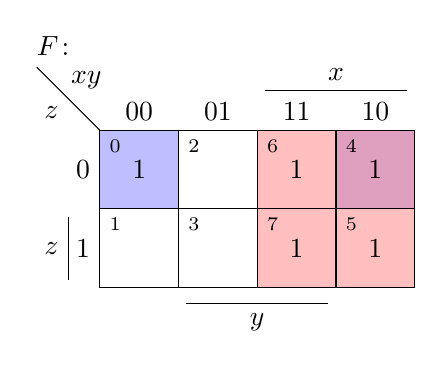
\begin{tikzpicture}
\karnaughmapcolorfield[fill]{3}{04}{blue!50}
\karnaughmapcolorfield[fill]{3}{6754}{red!50}
\karnaughmap[variables={xyz}, function={F}]{1000 1111};
\end{tikzpicture}\\~\\
$\ol{xyz}+x\ol{yz}$\\
$\ol{yz}(\cancel{\ol{x}+x}^1)$\\
$\ol{yz}$\\~\\
\begin{tabular}{cc}
110 & xy$\ol{z}$\\
100 & x$\ol{yz}$\\
111 & xyz\\
101 & x$\ol{y}$z\\
\end{tabular} If it's the same, it stays, but if it changes it goes.\\~\\
\answer{$F=\ol{yz}+x$}
\item Problem 12.1.5: Find the simplified SOP for $F=\sum_{x,y,z}(0,1,4,5,7)$ using a K-Map.\\
Distinguished 1's: 0, 1, 4, 7\\
Essential prime implicant: $\ol{y}$, $xz$\\~\\
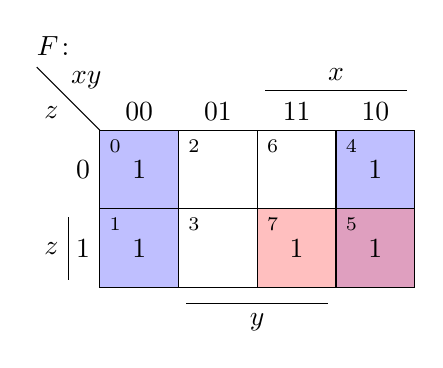
\begin{tikzpicture}
\karnaughmapcolorfield[fill]{3}{0145}{blue!50}
\karnaughmapcolorfield[fill]{3}{57}{red!50}
\karnaughmap[variables={xyz}, function={F}]{1100 1101};
\end{tikzpicture}\\~\\
\answer{$F=\ol{y}+xz$}
\end{itemize}
\subsection{Assigned Reading}
\begin{itemize}
\item Read 3.3.
\end{itemize}
\pagebreak
\section{2/24/2020}
\subsection{Lecture Slides}
\begin{itemize}
\item 
\end{itemize}
\subsection{Assigned Reading}
\begin{itemize}
\item 
\end{itemize}
\end{document}